%% abtex2-modelo-trabalho-academico.tex, v-1.7.1 laurocesar
%% Copyright 2012-2013 by abnTeX2 group at http://abntex2.googlecode.com/ 
%%
%% This work may be distributed and/or modified under the
%% conditions of the LaTeX Project Public License, either version 1.3
%% of this license or (at your option) any later version.
%% The latest version of this license is in
%%   http://www.latex-project.org/lppl.txt
%% and version 1.3 or later is part of all distributions of LaTeX
%% version 2005/12/01 or later.
%%
%% This work has the LPPL maintenance status `maintained'.
%% 
%% The Current Maintainer of this work is the abnTeX2 team, led
%% by Lauro César Araujo. Further information are available on 
%% http://abntex2.googlecode.com/
%%
%% This work consists of the files abntex2-modelo-trabalho-academico.tex
%% abntex2-modelo-include-comandos and abntex2-modelo-references.bib
%%

% ------------------------------------------------------------------------
% ------------------------------------------------------------------------
% abnTeX2: Modelo de Trabalho Academico (tese de doutorado, dissertacao de
% mestrado e trabalhos monograficos em geral) em conformidade com 
% ABNT NBR 14724:2011: Informacao e documentacao - Trabalhos academicos -
% Apresentacao
% ------------------------------------------------------------------------
% ------------------------------------------------------------------------

\documentclass[
	% -- opções da classe memoir --
	12pt,				% tamanho da fonte
	openright,			% capítulos não começam em pág ímpar (insere página vazia caso preciso)
	twoside,			% para impressão em verso e anverso. Oposto a oneside
	a4paper,			% tamanho do papel. 
	% -- opções da classe abntex2 --
	chapter=TITLE,		% títulos de capítulos convertidos em letras maiúsculas
	%section=TITLE,		% títulos de seções convertidos em letras maiúsculas
	%subsection=TITLE,	% títulos de subseções convertidos em letras maiúsculas
	%subsubsection=TITLE,% títulos de subsubseções convertidos em letras maiúsculas
	% -- opções do pacote babel --
	english,			% idioma adicional para hifenização
	french,				% idioma adicional para hifenização
	spanish,			% idioma adicional para hifenização
	brazil,				% o último idioma é o principal do documento
	hyphens,
  oldfontcommands]{abntex2}


% ---
% PACOTES
% ---

% ---
% Pacotes fundamentais 
% ---
\usepackage{cmap}				% Mapear caracteres especiais no PDF
\usepackage{lmodern}			% Usa a fonte Latin Modern			
\usepackage[T1]{fontenc}		% Selecao de codigos de fonte.
\usepackage[utf8]{inputenc}		% Codificacao do documento (conversão automática dos acentos)
\usepackage{minted}
\usepackage{lastpage}			% Usado pela Ficha catalográfica
\usepackage{indentfirst}		% Indenta o primeiro parágrafo de cada seção.
\usepackage{color}				% Controle das cores
\usepackage{graphicx}			% Inclusão de gráficos
\usepackage{soul}
\usepackage{gensymb}
\usepackage[version=4]{mhchem}
\usepackage{pdflscape}
\usepackage{afterpage}
\usepackage{capt-of}
\usepackage{subcaption}
\usepackage{helvet}
\renewcommand{\familydefault}{\sfdefault}
% ---

% ---		
% Posicionar os floats
% ---
\usepackage[bottom]{footmisc}
% http://tex.stackexchange.com/questions/62720/vertical-space-after-algorithm
% \setlength{\textfloatsep}{1.241\onelineskip}% Remove \textfloatsep
% \setlength{\floatsep}{1.241\onelineskip}% Remove \textfloatsep
% \setlength{\intextsep}{1.241\onelineskip}% Remove \textfloatsep
\setlength{\textfloatsep}{1\baselineskip}% Remove \textfloatsep
%\setlength{\floatsep}{1\baselineskip}% Remove \textfloatsep
%\setlength{\intextsep}{1\baselineskip}% Remove \textfloatsep
		
% ---
% Pacotes adicionais
% ---
\usepackage{lipsum}				% para geração de dummy text
\usepackage{siunitx}            % sistema internacional de unidades
\usepackage{amsmath,amssymb,amsthm} % pacotes matemáticos
\usepackage{pifont}             % para alguns símbolos especiais
\usepackage[version=4]{mhchem}  % fórmulas químicas
\usepackage{tabularx}
%\usepackage{listings}           % para os códigos
\usepackage{multirow}           % para agrupar linhas em colunas
\usepackage{pdfpages}
% ---

\usepackage{amsthm}
\usepackage{amsmath}
\usepackage{amssymb}
\usepackage{amsbsy}
\usepackage{esint}
\usepackage{bm}
\usepackage{float}
% This will add the units
%----------------------------------------------
\newcommand{\nomunit}[1]{%
\renewcommand{\nomentryend}{\hspace*{\fill}#1}}
%----------------------------------------------
 
\usepackage[most]{tcolorbox}
\usepackage[a4paper, total={6in, 8in}]{geometry}
%---
% Pacotes de citações
% ---
\usepackage[brazilian,hyperpageref]{backref}	 % Paginas com as citações na bibl
\usepackage[alf,abnt-etal-text=it,bibjustif]{abntex2cite}	% Citações padrão ABNT

% --- 
% CONFIGURAÇÕES DE PACOTES
% --- 

% ---
% Configurações do pacote backref
% Usado sem a opção hyperpageref de backref
\renewcommand{\backrefpagesname}{Citado na(s) página(s):~}
% Texto padrão antes do número das páginas
\renewcommand{\backref}{}
% Define os textos da citação
\renewcommand*{\backrefalt}[4]{
	\ifcase #1 %
		Nenhuma citação no texto.%
	\or
		Citado na página #2.%
	\else
		Citado #1 vezes nas páginas #2.%
	\fi}%
\usemintedstyle{monokai}
\definecolor{bg}{HTML}{282828}
\tcbset{theostyle/.style={
    enhanced,
    sharp corners,
    attach boxed title to top left={
      xshift=-1mm,
      yshift=-4mm,
      yshifttext=-1mm
    },
    top=1.5ex,
    colback=white,
    colframe=black,
    fonttitle=\bfseries,
    boxed title style={
      sharp corners,
    size=small,
    colback=black,
    colframe=black,
  } 
}}

\newtcbtheorem[number within=section]{Definition}{Definição}{%
  theostyle
}{def}

\theoremstyle{definition}
\newtheorem{definition}{Definition}
\newcommand{\R}{\bm{\mathrm{R}}}
\newcommand{\C}{\bm{\mathrm{C}}}
\newcommand{\Q}{\bm{\mathrm{Q}}}
\newcommand{\N}{\bm{\mathrm{N}}}
\newcommand{\Z}{\bm{\mathrm{Z}}}
\newcommand{\Pspace}{\bm{\mathrm{P}}}
\newcommand{\F}{\bm{\mathrm{F}}}
\newcommand{\fvec}{\bm{\mathrm{F}}}
\newcommand{\nvec}{\bm{\mathrm{n}}}
\newcommand{\vvec}{\bm{\mathrm{v}}}
\newcommand{\Svec}{\bm{\mathrm{S}}}
\newcommand{\wvec}{\bm{\mathrm{w}}}
\newcommand{\rvec}{\bm{\mathrm{r}}}
\newcommand{\xvec}{\bm{\mathrm{x}}}
\newcommand{\uvec}{\bm{\mathrm{u}}}
\newcommand{\bvec}{\bm{\mathrm{b}}}
\newcommand{\ivec}{\bm{\mathrm{i}}}
\newcommand{\jvec}{\bm{\mathrm{j}}}
\newcommand{\evec}{\bm{\mathrm{e}}}
\newcommand{\Jvec}{\bm{\mathrm{J}}}
\newcommand{\kvec}{\bm{\mathrm{k}}}
\newcommand{\zerovec}{\bm{\mathrm{zero}}}
\DeclareMathOperator{\spn}{span}

%\usepackage[margin=1cm]{geometry}
\theoremstyle{definition}
% ---

%%% -----
%%% Formato de cabeçalho/rodapé romano nos elementos pré-textuais
%%% -----

%% Novo estilo
\makepagestyle{estilo_pretextual} %%% escolha um nome
  \makeevenhead{estilo_pretextual}{}{}{\ABNTEXfontereduzida \textbf \thepage}
  \makeoddhead{estilo_pretextual}{}{}{\ABNTEXfontereduzida \textbf \thepage}

%% Customiza comando \pretextual
\renewcommand{\pretextual}{
  \pagenumbering{roman} %%% ou \pagenumbering{Roman}
  \aliaspagestyle{chapter}{estilo_pretextual}% customizing chapter pagestyle
  \pagestyle{estilo_pretextual}
  \aliaspagestyle{cleared}{empty}
  \aliaspagestyle{part}{estilo_pretextual}
}
\renewcommand{\ABNTEXchapterfontsize}{\normalsize\bfseries} %12pt
\renewcommand{\ABNTEXsectionfontsize}{\normalsize}
\renewcommand{\ABNTEXsubsectionfontsize}{\normalsize} 
% ---
% Ajusta a marca \textual para que a numeração volte a ser arábica
% nos elementos textuais
\let\oldtextual\textual        % copia o comando \textual anterior para \oldtextual
\renewcommand{\textual}{%
  \oldtextual%
  \pagenumbering{arabic} % volta à numeração arábica
}
% ---

% ---
% Informações de dados para CAPA e FOLHA DE ROSTO
% ---
\titulo{Uso de um modelo numérico para a otimização das curvas de secagem de concretos aluminosos}
\autor{Murilo Henrique Moreira}
\local{São Carlos -- SP}
\data{2019}
\orientador{Prof. Victor Carlos Pandolfelli}
\coorientador{Prof. Ana Paula Luz}
\instituicao{%
  Universidade Federal de São Carlos
  \par
  Centro de Ciências Exatas e de Tecnologia
  \par
  Departamento de Engenharia de Materiais}
\tipotrabalho{Trabalho de Conclusão de Curso (Graduação)}
% O preambulo deve conter o tipo do trabalho, o objetivo, 
% o nome da instituição e a área de concentração 
\preambulo{Trabalho de conclusão de curso apresentado ao curso de Engenharia de Materiais da Universidade Federal de São Carlos, como requisito parcial à obtenção do título de Bacharel em Engenharia de Materiais. Área de concentração: Cerâmicas.}
% ---

% ---
% Nova capa
% ---
\renewcommand{\imprimircapa}{%
\begin{capa}%
\center
\large\imprimirinstituicao
\par
\vspace*{3cm}
{\large\imprimirautor}\par
\vspace*{3cm}
{\ABNTEXchapterfont\bfseries\large\MakeUppercase\imprimirtitulo}
\vfill
\large\imprimirlocal
\par
\large\imprimirdata
\end{capa}
}
% ---
% Nova folha de rosto
% ---
\makeatletter
\renewcommand{\folhaderostocontent}{
\thispagestyle{empty}
\begin{center}
{\large\imprimirautor}
\vfill
{\ABNTEXchapterfont\bfseries\large\MakeUppercase\imprimirtitulo}\\
\vspace*{3cm}
\abntex@ifnotempty{\imprimirpreambulo}{%
\hspace{.45\textwidth}
\begin{minipage}{.5\textwidth}
\SingleSpacing
\imprimirpreambulo\\
\par
\imprimirorientadorRotulo~\imprimirorientador
\par
\imprimircoorientadorRotulo~\imprimircoorientador
\end{minipage}%
\vfill
}%
{\large\imprimirlocal}
\par
{\large\imprimirdata}
\end{center}
}
\makeatother
% ---

% ---
% Configurações de aparência do PDF final

% alterando o aspecto da cor azul
\definecolor{blue}{RGB}{41,5,195}

% informações do PDF
\makeatletter
\hypersetup{
     	%pagebackref=true,
		pdftitle={\@title}, 
		pdfauthor={\@author},
    	pdfsubject={\imprimirpreambulo},
	    pdfcreator={LaTeX with abnTeX2},
		pdfkeywords={abnt}{latex}{abntex}{abntex2}{trabalho acadêmico}, 
		colorlinks=true,       		% false: boxed links; true: colored links
    	linkcolor=black,          	% color of internal links
    	citecolor=black,        		% color of links to bibliography
    	filecolor=magenta,      		% color of file links
		urlcolor=blue,
		bookmarksdepth=4
}
\makeatother
% --- 

% --- 
% Espaçamentos entre linhas e parágrafos 
% --- 

% O tamanho do parágrafo é dado por:
\setlength{\parindent}{1.3cm}

% Controle do espaçamento entre um parágrafo e outro:
\setlength{\parskip}{0.2cm}  % tente também \onelineskip

% ---
% compila o indice
% ---
\makeindex
% ---

% ----
% Início do documento
% ----
\begin{document}

% Retira espaço extra obsoleto entre as frases.
\frenchspacing 

% ----------------------------------------------------------
% ELEMENTOS PRÉ-TEXTUAIS
% ----------------------------------------------------------
\pretextual

% ---
% Capa
% ---
\imprimircapa
% ---

% ---
% Folha de rosto
% (o * indica que haverá a ficha bibliográfica)
% ---
\imprimirfolhaderosto
% ---

% ---
% Inserir a ficha bibliografica
% ---

% Isto é um exemplo de Ficha Catalográfica, ou ``Dados internacionais de
% catalogação-na-publicação''. Você pode utilizar este modelo como referência. 
% Porém, provavelmente a biblioteca da sua universidade lhe fornecerá um PDF
% com a ficha catalográfica definitiva após a defesa do trabalho. Quando estiver
% com o documento, salve-o como PDF no diretório do seu projeto e substitua todo
% o conteúdo de implementação deste arquivo pelo comando abaixo:
%
\begin{fichacatalografica}
    \includepdf{ficha.pdf}
\end{fichacatalografica}
%\begin{fichacatalografica}
%	\vspace*{\fill}					% Posição vertical
%	\hrule							% Linha horizontal
%	\begin{center}					% Minipage Centralizado
%	\begin{minipage}[c]{12.5cm}		% Largura
	
%	\imprimirautor
	
%	\hspace{0.5cm} \imprimirtitulo  / \imprimirautor. --
%	\imprimirlocal, \imprimirdata-
	
%	\hspace{0.5cm} \pageref{LastPage} p. : il. (algumas color.) ; 30 cm.\\
	
%	\hspace{0.5cm} \imprimirorientadorRotulo~\imprimirorientador\\
	
%	\hspace{0.5cm}
%	\parbox[t]{\textwidth}{\imprimirtipotrabalho~--~\imprimirinstituicao,
%	\imprimirdata.}\\
	
%	\hspace{0.5cm}
%		1. Cerâmicas macroporosas.
%		2. Espumas.
%		3. Arduino.
%		I. Victor Carlos Pandolfelli.
%		II. Universidade Federal de São Carlos.
%		III. Centro de Ciências Exatas e de Tecnologia.
%		IV. Departamento de Engenharia de Materiais
%		V. Título\\ 			
	
%	\hspace{8.75cm} CDU 02:141:005.7\\
	
%	\end{minipage}
%	\end{center}
%	\hrule
%\end{fichacatalografica}
% ---

% ---
% Inserir errata
% ---
%\begin{errata}
%Elemento opcional da \citeonline[4.2.1.2]{NBR14724:2011}. Exemplo:

%\vspace{\onelineskip}

%FERRIGNO, C. R. A. \textbf{Tratamento de neoplasias ósseas apendiculares com reimplantação de enxerto ósseo autólogo autoclavado associado ao plasma rico em plaquetas}: estudo crítico na cirurgia de preservação de membro em cães. 2011. 128 f. Tese (Livre-Docência) - Faculdade de Medicina Veterinária e Zootecnia, Universidade de São Paulo, São Paulo, 2011.

%\begin{table}[htb]
%\center
%\footnotesize
%\begin{tabular}{|p{1.4cm}|p{1cm}|p{3cm}|p{3cm}|}
%  \hline
%   \textbf{Folha} & \textbf{Linha}  & \textbf{Onde se lê}  & \textbf{Leia-se}  \\
%    \hline
%    1 & 10 & auto-conclavo & autoconclavo\\
%   \hline
%\end{tabular}
%\end{table}

%\end{errata}
% ---

% ---
% Inserir folha de aprovação
% ---

% Isto é um exemplo de Folha de aprovação, elemento obrigatório da NBR
% 14724/2011 (seção 4.2.1.3). Você pode utilizar este modelo até a aprovação
% do trabalho. Após isso, substitua todo o conteúdo deste arquivo por uma
% imagem da página assinada pela banca com o comando abaixo:
%
% \includepdf{folhadeaprovacao_final.pdf}
%
% \begin{folhadeaprovacao}
% \thispagestyle{empty}
%   \begin{center}
%     {\large\imprimirautor}

%     \vfill
%     {\ABNTEXchapterfont\bfseries\large\MakeUppercase\imprimirtitulo}
%     \vfill
    
%     \hspace{.45\textwidth}
%     \begin{minipage}{.5\textwidth}
%         \imprimirpreambulo
%     \end{minipage}%
%     \vfill
%    \end{center}
    
%    Trabalho aprovado. \imprimirlocal, 28 de junho de 2018:

%    \assinatura{\textbf{\imprimirorientador}} 
%    \assinatura{\textbf{Márcio Raymundo Morelli}}
%    %\assinatura{\textbf{Professor} \\ Convidado 2}
%    %\assinatura{\textbf{Professor} \\ Convidado 3}
%    %\assinatura{\textbf{Professor} \\ Convidado 4}
    
%     \vfill  
%    \begin{center}
%     {\large\imprimirlocal}
%     \par
%     {\large\imprimirdata}
%   \end{center}
  
% \end{folhadeaprovacao}
% ---

% ---
% Dedicatória
% ---
\begin{dedicatoria}
   \vspace*{\fill}
   \centering
   \noindent
   \textit{Dedico esse trabalho aos meus pais, amigos e todos aqueles que me inspiram.} \vspace*{\fill}
\end{dedicatoria}
% ---

% ---
% Agradecimentos
% ---
\begin{agradecimentos}

Agradeço primeiramente aos meus pais, Margaret e Luiz Henrique Moreira, por todo o ensino de
responsabilidade e disciplina essenciais para alcançar meus objetivos, além do
carinho e amizade. Agradeço a minha irmã pelo exemplo de profissional dedicada e
perseverante durante uma belíssima vida acadêmica, com quem sempre pude
compartilhar os desafios de anos de IC. À minha companheira e melhor amiga
Mariana, pelo suporte, atenção e ajuda em todos os momentos, me mantendo firme
na Fé de que o melhor há de acontecer.

Agradeço ao Departamento de Engenharia de Materiais, pela qualidade de ensino e
inspiração que tanto professores reconhecidos proporcionaram e proporcionam.

Ao Prof. Pandolfelli pela orientação cuidadosa ao longo de 5 anos de graduação, que sempre
auxiliou e ajudou as melhores tomadas de decisão, sendo um verdadeiro mentor e proporcionando
crescimento profissional e pessoal, estando sempre disponível para ajudar com
paciência e humildade. Seu comprometimento com a ciência aplicada em tecnologia
é algo que inspira a mim e tantos outros, além de dever inspirar muitos de
nossos Professores Universitários deste país.

Agradeço especialmente à minha coorientadora, Prof. Ana Paula, por todos os
ensinamentos e auxílio na parte experimental sem a qual toda a simulação se
tornaria irrelevante, além das ideias e da grande amizade.

Também agradeço ao Professor Roberto Frederico Ausas por todo ensinamento e
auxílio com os métodos numéricos e com as profundas análises do problema, tanto
do ponto de vista dimensional, quanto do ponto de vista de implementação, e
também ao Mestre Pedro Ivo Pelissari pela ajuda e auxílio nas fases preliminares
do projeto.

Agradeço também a todos do Grupo de Engenharia de Microestrutura de Materiais,
pelo suporte e parceria nas pessoas do técnico Guilherme Morbiolli, ao Mestre
Matheus Felipe Santos e ao Graduando Túlio Mumi\'c Cunha e todos os outros
colegas que tornaram o dia a dia sempre mais amistoso.

E finalmente ao Professor Ricardo Afonso Angélico que me introduziu no mundo dos elementos
finitos com a maior das didáticas, deixando claro que sempre há uma maneira
lógica, metódica e correta de se trabalhar com simulação computacional,
inspiro-me em um dia ter tamanha competência em compartilhar tantos assuntos
complexos de maneira simples.

E aos meus amigos e colegas de curso, com os quais compartilho grandes memórias,
Rodrigo, Murilo, Denis, Augusto e tantos outros. 

\end{agradecimentos}
% ---

% ---
% Epígrafe
% ---
\begin{epigrafe}
    \vspace*{\fill}
	\begin{flushright}
		\textit{``Simplicidade é a conquista final.\\ Depois de uma vasta quantidade
      de notas e mais notas, \\ é a simplicidade que surge como a recompensa
      máxima da arte.''\\
		Frédéric Chopin}
	\end{flushright}
\end{epigrafe}
% ---

% ---
% RESUMOS
% ---

% resumo em português
\begin{resumo}


 \vspace{\onelineskip}
    
 \noindent
 A etapa de secagem de concretos refratários é um dos pontos principais durante
 a aplicação deste tipo de material. Um aquecimento muito rápido pode levar o
 material a trincar ou ainda explodir, devido a pressurização do vapor de água
 que estava previamente adsorvido fisicamente e também ligado quimicamente nas
 fases presentes na microestrutura. Assim, é comum nas indústrias o uso de
 curvas de secagem essencialmente empíricas, demasiadamente conservadoras, o que
 leva em um aumento do tempo improdutivo de reparo ou de construção do
 equipamento, um maior gasto de combustíveis fósseis e uma redução da
 competitividade financeira do usuário. Assim, o uso de modelos computacionais
 capazes de simular a secagem de revestimentos cerâmicos densos prevendo os
 campos de pressão do vapor de água no interior da microporosidade, se faz
 extremamente útil. Tais modelos já são utilizados na avaliação de concretos
 para a construção civil, porém seu desenvolvimento resultou em modelos
 complicados e dependentes de inúmeras propriedades e de ensaios complexos.
 Assim, o presente trabalho buscou a obtenção de um modelo capaz de ser
 utilizado para a otimização de curvas de secagem de concretos aluminosos
 ligados com cimento de aluminado de cálcio. Tal objetivo foi atingido ao se
 utilizar de informações coletadas nos ensaios de termogravimetria para a
 obtenção das curvas de sorção isotérmica. Em seguida, através de um controlador
 Proporcional Integral Derivativo foi possível otimizar uma curva de secagem
 similar às utilizadas na indústria, reduzindo as pressões no interior do
 material no mesmo intervalo de tempo.
 
 \textbf{Palavras-chaves}: Concretos Refratários, Explosão, Modelo Numérico, FEM, FEniCS.
\end{resumo}

% resumo em inglês
\begin{resumo}[Abstract]
\begin{otherlanguage*}{english}
\vspace{\onelineskip}

\noindent
The drying step of refractory concretes is one of the main points during the
application of this type of material. A very fast heating may lead the material
to crack or even explode due to the pressurization of the water vapor which was
previously physically adsorbed and also chemically bound in the present phases
of the cured material. Thus, it is common to use essentially empirical drying
curves on the industry, generally over conservative, which leads to an increase
in the repair time of the equipment, an increase on the spending of fossil fuels
and a reduction of the financial competitiveness of the end user. Therefore, the
use of models to simulate the drying by predicting the pressure fields of the
water vapor inside the microporosity becomes extremely useful. Such models are
already used in the civil construction field, but its development resulted in
complex models dependent on numerouss properties and complex tests. Hence, the
present study aimed obtain a model capable of being used for the
optimization of the drying curve. This objective was accomplished when using the
thermogravimetry analysis to adjust the isothermal sorption curves. Then,
through a Proportional Integral Derivative controller it was possible to
optimize a fiction heat up curve similar to the ones used in industry and to
reduce the pressure inside the material using the same time.

   \textbf{Keywords}: Refractory Castable, Spalling, Numerical Model, FEM, FEniCS.
   
 \end{otherlanguage*}
\end{resumo}

% resumo em francês 
%\begin{resumo}[Résumé]
% \begin{otherlanguage*}{french}
%    Il s'agit d'un résumé en français.
 
%   \vspace{\onelineskip}
 
%   \noindent
%   \textbf{Mots-clés}: latex. abntex. publication de textes.
% \end{otherlanguage*}
%\end{resumo}

% resumo em espanhol
%\begin{resumo}[Resumen]
% \begin{otherlanguage*}{spanish}
%   Este es el resumen en español.
  
%   \vspace{\onelineskip}
 
%   \noindent
%   \textbf{Palabras clave}: latex. abntex. publicación de textos.
% \end{otherlanguage*}
%\end{resumo}
% ---

% ---
% inserir lista de ilustrações
% ---
\pdfbookmark[0]{\listfigurename}{lof}
\listoffigures*
\cleardoublepage
% ---

% ---
% inserir lista de tabelas
% ---
\pdfbookmark[0]{\listtablename}{lot}
\listoftables*
\cleardoublepage
% ---

% ---
% inserir lista de abreviaturas e siglas
% ---
\begin{siglas}
  \item[TGA] Análise Termogravimétrica
  \item[DTG] Derivada da curva de perda de massa
  \item[PTM] Ensaio de aquecimento unilateral com medidas de pressão,
    temperatura e massa
  \item[OSH] Ensaio equivalente ao PTM
  \item[FEM] Método dos elementos finitos
  \item[P1]  Elemento polinomial linear
  \item[PID] Controlador Proporcional integral derivativo
\end{siglas}

% ---
% inserir lista de símbolos
% ---
\begin{simbolos}
  \item[$ t $] Tempo, $s$
  \item[$ T $] Temperatura, $^{\circ}C$
  \item[$ P_v $] Pressão devido ao vapor no interior do material, $Pa$
  \item[$ h $] Coeficiente de transferência de calor, $W \ m^{-2} \
    ^{\circ}C^{-1}$
  \item[$ h_m $] Coeficiente de transferência de massa, $s m^{-1}$
  \item[$ w $] Curvas de Sorção Isotérmicas, $kg \ m^3$
  \item[$ C_p $] Calor específico do concreto, $J \ \kg^{-1} \ K^{-1}$
  \item[$ \rho $]  Densidade do concreto, $kg \ m^{-1}$
  \item[$ \C_w $]  Calor específico da àgua, $J \ \kg^{-1} \ K^{-1}$
  \item[$ \C_a $] Calor latente de evaporação da água $J \ kg^{-1}$
  \item[$ \lambda $] Condutividade térmica, $W \ m^{-1} \ ^{\circ}C^{-1}$
  \item[$ \Omega $] Domínio do modelo, $-$ 
  \item[$ \Gamma_D $] Contorno sujeito a uma condição de contorno de Dirichlet, $-$
  \item[$ \Gamma_N $] Contorno sujeito a uma condição de contorno de Robin ou
    Neumann, $-$
  \item[$ \psi $] Função Teste, $-$
  \item[$ g $] Aceleração da gravidade, $m \ s^{-2}$
  \item[$ \mathbf{n} $] Vetor normal à superfície, $-$
  \item[$ w_0 $]  Massa de água para saturação de concreto a temperatura
    ambiente, por $kg$ de concreto, $kg \ m^{-3}$
  \item[$ w_c $]  Massa de cimento por $m^3$ de concreto, $kg \ m^{-3}$
  \item[$ \Delta T $] Aumento da temperatura na face quente obtida pelo
    controlador PID, $ ^{\circ}C $ 
  \item[$ K_p $] Coeficiente do termo proporcional do controlador PID, $-$
  \item[$ K_i $] Coeficiente do termo integral do controlador PID, $ s^{-1} $
  \item[$ K_d $] Coeficiente do termo derivativo do controlador PID, $ s $
  \item[$ e $] Diferença entre a pressão entre a máxima pressão no tempo $ t $ e a
    pressão de limite, $ Pa $
  \item[$ \tau $] Variável de integração com respeito ao tempo 
  \item[$ P_v^{max} $] Pressão máxima no tempo $t$, $ Pa $
  \item[$ \sigma_f $] Resistência mecânica à flexão 3 pontos, $MPa$
    
\end{simbolos}

%---

% ---
% inserir o sumario
% ---
\pdfbookmark[0]{\contentsname}{toc}
\tableofcontents*
% ---



% ------------------------------
% \end{document}
% ----------------------------
% ELEMENTOS TEXTUAIS
% ----------------------------------------------------------
\textual

% ----------------------------------------------------------
% Introdução
% ----------------------------------------------------------
\chapter{Introdução} \label{introducao}
\section{Apresentação do problema}
   Materiais refratários monolíticos são materiais fornecidos pelo o produtor
   sem um formato específico, podendo ter sua conformação feita pelo consumidor. Tais
   materiais apresentam inúmeras vantagens como uma maior facilidade de
   aplicação quando comparado com os materiais conformados, possibilidade de uso
   como material de reparo, e conformação de geometrias complexas.

   Porém, a etapa de queima é a principal desvantagem que essa
   categoria de materiais refratários apresenta. Tal processo exige uma queima
   lenta e cautelosa para liberar a água física e quimicamente ligada sem causar
   danos ao material. O fator de segurança para designar as curvas de
   aquecimento é comumente demasiadamente conservador, motivado pelo risco que
   uma queima má realizada apresenta de levar ao aparecimento de trincas, lascamentos e até mesmo a explosão de todo o revestimento, ou ainda, de todo o equipamento,
   conforme ilustrado na Figura \ref{fig:spalls}.
    
    \begin{figure}[ht]
        \centering
        \includegraphics[width=0.7\textwidth]{figures/spallings.pdf}
        \caption{Casos de explosão decorrente de curvas de secagem em um
          calcinador de alumina (a), no teto de um forno de alumínio (b), no
          funil de alimentação de um alto-forno (c), em um duto de gás do
          alto-forno (d). Editado de \cite{irish}}
        \label{fig:spalls}
   \end{figure}

   As dificuldades em se obter uma curva de secagem otimizada se relacionam com
   a ausência de uma metodologia que considere toda a complexidade decorrente da
   interação de diversos fatores como as condições ambientais, a geometria do
   dispositivo, o transporte de calor na peça, o transporte de massa, as
   mudanças de fase e as propriedades pertinentes em função do tempo. Sendo
   assim, o procedimento padrão se dá através da obtenção empírica das curvas de
   secagem usando comumente uma combinação de rampas e patamares conforme
   apresentado na Figura \ref{fig:hucs}.
      
    \begin{figure}[ht]
        \centering
        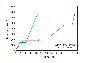
\includegraphics[width=0.7\textwidth]{figures/hucs.pdf}
        \caption{Exemplos de curvas de secagem comumente utilizadas. Retirado de \cite{rhi}}
        \label{fig:hucs}
   \end{figure}

   Portanto, o problema que o presente trabalho aborda é como usar ferramentas
   matemáticas para modelar os fenômenos de transporte de massa e calor que
   ocorrem durante a secagem para contribuir no entendimento desse complexo
   fenômeno e possibilitar que otimizações sejam realizadas tornando tal processo mais eficiente em termos de tempo e de consumo energético contribuindo para a redução dos custos financeiros e ambientais que tal processo inflige atualmente.
 
 A existência de ferramentas computacionais para a simulação de tal processo derivam de trabalhos baseados nos estudo de concretos de construção civil sujeitos a altas temperaturas em reatores nucleares ou em construções em incêndio.  Esses modelos podem considerar inúmeros processos simultâneos, o que eleva sua complexidade. Sendo assim, um desafio abordado no presente trabalho é tornar usar simplificações que possibilitem o uso de tais ferramentas em aplicações refratárias.
   
\section{Objetivos}
    \subsection{Objetivo geral}
        
    Desenvolver e implementar um modelo numérico que considere o menor número possível de parâmetros para poder prever a secagem de materiais refratários monolíticos, utilizando o ensaio de termogravimetria (TGA) para realizar a validação da simulação numérica.
        
    \subsection{Objetivos específicos}
        
    \begin{itemize}
        \item Realizar uma revisão bibliográfica sobre as metodologias de otimização de curvas de secagem;
        
        \item Desenvolver um modelo capaz de simular os resultados do ensaio de termogravimetria utilizando apenas soluções \textit{open source};
        
        \item Realizar o \textit{benchmarking} do modelo com os dados do ensaio;
        
        \item Retirar \textit{insights} do modelo e explorar casos de estudo.
    \end{itemize}
        
\section{Motivação}
   Materiais refratários são fundamentais nas principais indústrias
   habilitadoras, isto é, indústrias que fornecem maneiras de manufaturar outros
   materiais. No caso, o processo siderúrgico, que é responsável por 5 \% \cite{Davis2018} da
   liberação de CO$_2$  está intimamente relacionado com a
   indústria de materiais refratários. Tal relação é tamanha que a qualidade dos
   aços produzidos dependem diretamente da qualidade do material refratário, que
   permite, por exemplo, reduzir  o teor de carbono das ligas, por exemplo. Além disso, embora os avanços da
   área tenham reduzido consideravelmente a quantidade de refratário consumida
   por tonelada de aço (chegando até o valor de 10kgs por tonelada de aço no Japão, esse valor é ainda expressivo e com potencial para redução em diferentes mercados (como no mercado Chinês, onde estima-se um consumo de 23kgs por tonelada de aço)  \cite{refperton}.

   Nesse contexto, ampliar a vida útil dos refratários, diminuir o impacto
   ambiental de sua instalação e otimizar os tempos de manutenção podem ter
   efeitos determinantes tanto em aspectos sócio-ambientais como também
   consequências financeiras que permitam investimentos e avanços em novos
   materiais, gerando um processo contínuo de ganho de eficiência.

   A simulação do processo de secagem influencia em todos esses aspectos de
   maneira direta ou indireta, através da redução dos danos proporcionados pela
   pressão de vapor gerado no interior do material, ampliando a vida útil do
   material, agilizando a remoção da água física e quimicamente ligada, acelerando os processos de secagem e reduzindo o consumo de energia para o
   primeiro aquecimento e diminuindo as curvas iniciais de secagem, permitindo
   um ganho de eficiência no processo de manutenção dos equipamentos.

   Além dos ganhos de otimização, um maior entendimento dos processos
   concorrentes que ocorrem durante a secagem podem oferecer novos \textit{insights} para
   soluções que consigam garantir uma relação otimizada de permeabilidade e
   resistência mecânica do material, duas propriedades fundamentalmente
   inversamente proporcionais.


\section{Resultados esperados} \label{results-esperados}
   Espera-se ao final desse projeto se ter um modelo capaz de simular
   numericamente o processo de secagem de um material refratário, validado
   através de ensaios baratos (sem necessitar de inúmeros termopares e transdutores de
   pressão) com um número reduzido de parâmetros, selecionados a partir de uma
   análise de sensibilidade.

   Através do uso de tal modelo, diversos estudos de caso funcionariam como
   forma de proporcionar \textit{insights} em como otimizar o processo de secagem dos
   materiais refratários monolíticos.

    
\section{Estrutura do trabalho}
    
Esta monografia encontra-se estruturada da seguinte forma:
    
\autoref{introducao} – apresenta a introdução do trabalho, seus objetivos, motivação e os resultados esperados;
    
\autoref{fundteorica} – descreve os conceitos de materiais refratários
monolíticos, apresentando suas principais características; avalia o estado da
arte das metodologias de controle e otimização empírica da remoção de água de
materiais refratários e por fim apresenta modelos gerais de secagem
    
\autoref{metodologia} – detalha os materiais e métodos utilizados no trabalho;
    
\autoref{results} – consiste na análise dos resultados obtidos tanto na caracterização das propriedades necessárias ao modelo bem como dos testes experimentais necessários para sua validação e por fim a comparação destes com os resultados numéricos discutindo-se as razões de seu funcionamento e das divergências;

\autoref{conclusao} – apresenta a conclusão do trabalho e algumas ideias para trabalhos futuros.
    
Ao final da monografia encontram-se as referências bibliográficas utilizadas, um apêndice apresentando detalhes do modelo matemático e outro contendo o programa desenvolvido na linguagem Python \cite{python}.

% ----------------------------------------------------------
% Fundamentação teórica
% ----------------------------------------------------------

\chapter{Fundamentação teórica} \label{fundteorica}
\section{Materiais Refratários Monolíticos}\label{mono}

	Os materiais refratários são componentes fundamentais nas economias modernas exercendo o papel de indústria habilitadora no sentido que possibilita a execução de processos a elevadas solicitações térmicas, químicas e mecânicas em um ambiente controlado e seguro. Ademais, o contexto sócio-ambiental do século XXI exige o máximo cuidado a fim de reduzir o desperdício de energia, especialmente de processos que ocorrem a altas temperaturas, onde a perda de energia para o ambiente é inerente.

	Assim, a indústria de materiais refratários está diretamente ligada a outras indústrias fundamentais como a indústria de cimento e principalmente a siderúrgica, ambas indústrias extremamente correlacionadas com o produto interno bruto (PIB) das nações, conforme demonstrado no gráfico temporal mostrado na Figura \ref{fig:refractory_economy}

\begin{figure}[ht]
\centering
\includegraphics[width=\linewidth]{./figures/refractory_economy.pdf}
\caption{Evolução temporal do PIB mundial (azul escuro, eixo esquerdo), da produção mundial de Aço e Cimento (azul e azul claro, eixo direito) no período de 1999 a 2015.  Adaptado de \cite{GlobalRef2017}. \label{fig:refractory_economy}}
\end{figure}
		Com esse papel fundamental, os materiais refratários (que também passam por processos em alta temperatura durante sua fabricação) também passam por uma mudança de paradigma relativamente recente, isto é, ao invés do produtor fornecer peças pré-formadas (refratários conformados), este passa a oferecer um material conformável (monolítico), o que otimiza a logística - do ponto de vista do produtor, evita e reduz estoques, reduz o custo energético e permite uma maior customização do produto por parte do comprador.
        
        Dessarte, a seguir é realizada uma breve revisão do conceito de materiais monolíticos explorando seu processamento e finalmente vantagens e desvantagens características de tal classe de materiais.

    \subsection{Conceito}
    
    Dentro da classe de materiais monolíticos, a classe dos concretos ("\textit{castables}") é uma das que mais evoluíram recentemente. Uma motivação para sua evolução é sua facilidade de aplicação que aliada aos avanços em automatização gerou um interesse enorme no potencial dessa classe de materiais refratários, além de sua performance avançada \cite{Schacht2004}. Tal classe compreende materiais compostos, no geral, por agregados, uma matriz, ligantes, materiais secundários e aditivos o que amplia sua possibilidade de ajuste de propriedades.
    Os agregados formam o "esqueleto" do material, sendo os componentes de maior teor mássico dentro das formulações. A matriz é composta por materiais mais finos que objetivam maximizar o empacotamento do material, enquanto o ligante é o componente que confere a resistência mecânica de fato. Os materiais secundários são componentes mais baratos que também auxiliam na otimização do empacotamento da composição enquanto os aditivos são responsáveis a atribuir características que possibilitem os mais diversos tipos de metodologia de aplicação, como aceleradores e retardantes de pega, dispersantes e controladores de pH.
    A complexidade da formulação permite ajustes específicos que podem alterar as propriedades finais do produto. Um exemplo é o uso de agregados leves e porosos como uma maneira de redução da condutividade térmica, proporcionando um isolante com alta resistência mecânica, ou ainda o uso de carbono como um material secundário, que devido sua baixa molhabilidade por metais líquidos aumenta a resistência a corrosão do produto \cite{Schacht2004}.
    Outro fator importante da formulação, e que recentemente passou a definir inclusive quais as quantias de cada fração granulométrica, é o seu grau de empacotamento. Como resistência a ambientes altamente reativos é uma propriedade inerente dos materiais cerâmicos, a redução da porosidade foi uma das grandes motivações que levaram a consideração de teorias de empacotamento para o ajuste da formulação. Dentre as principais, listam-se a teoria de empacotamento de Alfred e o modelo de Andreasen \cite{Ortega1997}. 
    Tais avanços permitiram materiais cuja resistência mecânica obtida fosse relativamente elevada. Entretanto, um dos grandes contrapontos à maximização do empacotamento se dá na etapa de secagem do material. Especialmente em concretos com ligações hídricas (como sistemas com CAC), reações de desidratação passam a ocorrer na faixa de 210$\degree$C à 370$\degree$C, o que pode gerar vapores aprisionados na estrutura pouco permeável das composições de empacotamento otimizado, sendo possível que os níveis de pressão alcançados nessas regiões sejam maiores que a resistência mecânica do material levando à trincamento, lascamento e até mesmo explosões.
    
    \subsection{Processamento}
      O processamento de materiais refratários monolíticos é altamente dependente da metodologia de aplicação a ser utilizada.


    \subsection{Vantagens e desvantagens}
      Capítulos 10 e 11 - Livro Ana
\section{Secagem de Refratários Monolíticos}\label{secagem}
De todas as etapas de processamento de materiais monolíticos com ligantes
hidráulicos, a secagem é uma das que mais toma tempo durante o processo de
reparo [REF LIVRO]. Devido a tal fator, há um grande potencial de ganho (em
termos de tempo de reparo e energia) na utilização de procedimentos de secagem
mais eficientes. Porém, qualquer dano provocado no material durante tal etapa
compromete a vida útil do refratário.

Além de tais desafios, garantir que a secagem, de fato, siga os procedimentos
recomendados pelo produtor (as curvas de secagem) é algo complexo dado
ineficiências do sistema de aquecimento (outro setor onde a simulação
computacional pode proporcionar grandes ganhos referentes a otimização do
sistema de aquecimento, bem como maior precisão e acurácia do sistema
controlador de temperaturas) e da falta de instrução dos operadores [REF LIVRO]. Soma-se o
fato de que muitas vezes as recomendações dadas pelo produtor são motivadas muito
mais pelo temor de ter que arcar com os custos de uma explosão ou de danos ao
equipamento devido problemas na secagem do que de fato fundamentos científicos e
testes experimentais.

Sendo assim há três estratégias comuns para a redução do risco de danos durante
o processo de secagem [REF LIVRO]:

\begin{enumerate}
\item Otimização da curva de secagem: \\ Para que a maior quantidade de água
  seja removida durante o regime de evaporação e não durante o regime de ebulição;
\item Alteração da microestrutura do material: \\ Para aumentar a permeabilidade e
  diminuir o nível de pressurização no interior do material;
\item Aumento da resistência mecânica: \\ Para que o material resista às tensões
  triaxiais decorrente da pressão do vapor de água.
\end{enumerate}

As próximas seções abordam cada uma dessas estratégias de forma mais
compreensiva, de forma a mostrar o estado da arte e como as simulações
computacionais poderiam complementar os estudos nesta área.

    \subsection{Curvas de secagem}
    Uma forma bastante comum no meio industrial para se definir uma curva de
    secagem é apresentado na Figura \ref{fig:industrial_HUC}.

\begin{figure}[ht]
\centering
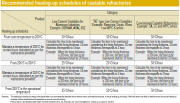
\includegraphics[width=\linewidth]{./figures/industrial_HUC.pdf}
\caption{Procedimento de secagem recomendado pela empresa AGC ceramics. Retirado de \cite{agc2016}. \label{fig:industrial_HUC}}
\end{figure}

    Observa-se que as taxas são definidas em diferentes intervalos de
    temperautra baseados aproximadamente nas temperautras de decomposição dos
    hidratos presentes no material. Além disso, o período de tempo em cada etapa
    é definido a partir da espessura do equipamento como uma maneira de se levar
    me consideração o efeito da distribuição de temperatura no interior do
    material.

    A crítica que se faz de tal procedimento é que tal correlação linear entre a
    temperatura e a espessura do componente não traduz os resultados
    experimentais e numéricos. Além disso, há a influência do próprio transporte
    de massa no interior do material nos perfis de temperatura o que pode gerar
    perfis completamente distintos.

    Tais orientações deveriam ser complementadas por resultados experimentais e
    simulações numéricas levando em conta não só as dimensões do refratário como
    também as condições de contorno, a geometria, a condutividade térmica e a
    permabilidade do material.

    Do ponto de vista empírico, ensaios de análise termogravimétrica podem ter
    grande importância para verificar se os intervalos de transofrmações
    propostos na curva de secagem, de fato correspondem com as trasnformações.

    \subsection{Aditivos para secagem}
     As recomendações 2 e 3 (alteração da microestrutura e aumento da
     resistência mecânica) podem ser implementadas através de aditivos
     adicionados na composição dos concretos. Dois casos específicos serão
     apresentados, são eles o uso de fibras poliméricas e fibras metálicas.
     Porém é importante salientar que inúmeras outras possibilidades também
     podem contribuir para o aumento de permeabilidade ou o aumento da
     resistência mecânica do material (como uso de diferentes sistemas ligantes,
     ou fases estabilizadas).

     As fibras metálicas apresentam a característica de ampliar a energia de
     fratura ao promover diferentes mecanismos de tenacificação como {\it
       crack-bridging}, {\it microcracking} e {\it pullout} [REF LIVRO]. Dessa
     maneira, há uma maior resistência ao dano por parte do material, de modo
     que as tensões devido a pressão do vapor não sejam capazes de promover o
     crescimento catastrófico das trincas. Além do efeito mecânico, o {\it
       microcracking} decorrente do {\it mismatch} dos coeficientes de expansão
     da matriz e das fibras metálicas, promove um aumento local da
     permeabilidade do material conforme reportado por Li et al \cite{li2019}.

     Por outro lado, as fibras poliméricas não apresentam quaisquer efeitos de
     tenacificação, inclusive promovendo defeitos de maiores dimenões o que
     diminui a resistêencia mecânica do material uma vez que tais polímeros são
     decompostos intencionalmente à baixas temperaturas (200$^\circ$C a
     300$^\circ$C) para promover o aumento da permeabiliade do material.

     Novamente, o uso da simulação computacional se faz importante uma vez que é
     necessário identificar a temperatura na qual a pressão no interior do
     material é máxima para selecionar o grade correto que apresente uma
     temperatura de composição coerente.

     Dessa forma justifica-se a busca por modelos númericos que possam garantir
     a otimização das curvas de secagem seja como um complemento às metodologias
     já sugeridas (como otimização da taxa de aquecimento, aumento da
     permebailidade ou aumento da resistência mecânica) ou ainda através de
     novas estratégias descobertas através da possibilidade de se obter os
     campos de pressão e temperatura no interior do material.
     
        
%%% Local Variables:
%%% mode: latex
%%% TeX-master: "TCC-Secagem"
%%% End:

\section{Modelos de Secagem}\label{modelos}
Inúmeros esforços estão sendo reportados na literatura para a simulação do fluxo
de fluídos em meios porosos, sendo que a secagem de concretos refratários é apenas uma das
inúmeras aplicações em que tal fenômeno é observado, havendo ainda
aplicações em tópicos de geofísica (movimentação de corpos hídricos em subsolo),
modelamento de poços de petróleo, e ainda simulações do comportamento de
estruturas de concreto em situações de incêndio (essa a aplicação mais próxima
na qual grande desenvolvimento tem sido realizado, ver \ref{sec:bazant}).


Os primeiros esforços para tais modelamentos foram realizados por Aleksei
Vasielivich Luikov \cite{martynenko2010} a partir de 1929. Devido ao uso ainda
incipiente de métodos numéricos, Luikov elaborou metodologias para a obtenção de
soluções analíticas para os problemas de transporte de massa e energia além de
trabalhos que propunham experimentos para validação de seus modelos, avançando
enormemente tal área do conhecimento \cite{Mikhailov1983}. Os modelos propostos
por Ba\v{z}ant e desenvolvido por outros autores nos últimos anos são derivados da
formulação de Luikov, documentada em seu Livro de 1964, ``\textit{Heat and Mass
  Transfer in Capillary Porous Bodies}'' \cite{luikov1964heat}.

Conforme descrito por Luikov, o transporte de massa dentro de uma matriz porosa
(como concretos, onde apesar de serem classificados como materiais densos
apresentam uma microporosidade conectada em sua microestrutura)
pode se dar tanto no estado gasoso quanto no estado líquido. No estado gasos o
fluxo se dá pelo movimento do vapor e da mistura de gases através da difusão a
nível molecular e molar através da filtração, isto é, o fluxo decorrente
da queda de pressão da mistura vapor-gás no interior do material. Já o movimento
do líquido pode decorrer também por difusão, filtração devido ao gradiente de
pressão ou ainda por absorção capilar nas camadas adsorvidas.

Os modelos subsequentes simplificam os fluxos por difusão e focam na descrição
do fluxo por filtração através da lei de Darcy. As seções seguintes descrevem os
modelos derivados das equações de Luikov.
    
    
\subsection{Modelo de Ba\v{z}ant}\label{sec:bazant}
Zedn\v{e}k Ba\v{z}ant é Professor de Engenharia Cívil e Engenharia de Materiais
da universidade de Northwestern reconhecido mundialmente pelos seus trabalhos em
mecânica dos sólidos em estruturas de concreto \cite{bundesen2004biography}. No
ínicio dos anos 70, Ba\v{z}ant estudou o efeito de altas temperaturas em
estruturas de concreto (contendo cimento Portland) para aplicações nucleares.
    
O modelo de Ba\v{z}ant se destaca por dois grandes motivos, primeiramente foi
vanguardista ao ser o primeiro (dos trabalhos encontrados durante a revisão
bibliográfica do presente trabalho) que utilizou de métodos numéricos para
resolver uma formulação simplificada das equações propostas por Luikov e, pelas
próprias simplificações utilizadas, que permitiram uma abordagem semi-empírica
direcionada com grande foco para a aplicação em questão. A presente seção usará
uma notação próxima à utilizada pelo autor, porém alguns termos serão adaptados
para conferir uma maior clareza e coerência com os modelos aqui utilizados.

A formulação de Ba\v{z}ant se inícia através da definição do fluxo mássico de
uma única fase que representa a água líquida, o vapor e o ar dentro do sistema,
obedecendo à da Lei de Darcy e do fluxo de Soret, e do fluxo de energia térmica
através da lei de Fourier e do fluxo de Dofour \cite{bazant1978thermal,
  bazant1978, bavzant1982, bazant1979}:

\begin{equation}
  \label{eq:Darcy}
  \vec{J}_{Darcy} = - \rho \vec{v} = - \rho \frac{\kappa }{\nu} \nabla P 
\end{equation}

\begin{equation}
  \label{eq:Soret}
  \vec{J}_{Soret} = - D_s \nabla T
\end{equation}

\begin{equation}
  \label{eq:Fourier}
  \vec{q}_{Fourier} = - \lambda \nabla T 
\end{equation}

\begin{equation}
  \label{eq:Dufour}
  \vec{q}_{Dufour} = - D_d \nabla P
\end{equation}

A simplificação do transporte mássico por uma única fase foi um dos pontos que
gerou uma certa cisão entre autores que adotaram tal prática, \cite{Gong1995a,
  Gong1991, Abdel-Rahman1996}, e outros que separaram cada componente,
\cite{Pesavento2013, Gawin2003, Gawin2004, Gawin1999, Fey2016b, Davie2006a,
  Davie2012a}, sendo este a parcela que mais se desenvolveu nos últimos anos.

Porém, Ba\v{z}ant defende que devido à morfologia dos canais pelos quais tais
fluidos passam, tal simplificação é coerente dado que o caminho livre médio das
moléculas de vapor (fase que seria mais móvel, em teoria) é maior que o
espaçamento entre os poros, e portanto sua movimentação se dá linearmente,
movendo consigo a camada de moléculas adsorvidas na superfície interna do
material \cite{bavzant2018creep}.

Uma vez definido tais fluxos as primeiras simplificações são feitas, os fluxos
de Soret ($\vec{J}_{Soret}$) e de Dufour ($\vec{q}_{Dufour}$) são considerados
desprezíveis devido resultados experimentais \cite{bazant1979}. Em
seguida, é considerada em uma equação de balanço energético, e outra de balanço
mássico gerando um sistema de equações parciais diferenciais.

\begin{equation}
  \label{eq:baz_MB}
  \underbrace{\frac{\partial w}{\partial t}}_{\text{(a)}} = \underbrace{\vphantom{ \left(\frac{a}{b}\right) } - \nabla \cdot \vec{J}_{Darcy}}_{\text{(b)}} + \underbrace{\frac{\partial w_d}{\partial t}}_{\text{(c)}}
\end{equation}

O termo $(a)$ da Equação \ref{eq:baz_MB} corresponde a taxa de liberação de água
livre do sistema em um dado ponto, sendo portanto equivalente à quantidade de
água transportada para (ou de) tal ponto, representado pelo termo (b), e a
quantidade de água liberada durante a desidratação (ou consumida durante a
hidratação), termo (c).

O balanço energético por sua vez se dá através da igualdade da taxa de consumo
(ou liberação de energia térmica) em dado ponto, Equação \ref{eq:baz_EB}, termo
$(a)$, com a taxa de consumo de energia para a liberação da água livre, termo
$(b)$, a quantidade de calor transportada por convecção, termo $(c)$ e a
quantidade de calor transportado por condução, termo $(d)$.

\begin{equation}
  \label{eq:baz_EB}
  \underbrace{\rho \ C_p \ \frac{\partial T}{\partial t}}_{\text{(a)}} = \underbrace{C_a \ \frac{\partial w}{\partial t}}_{\text{(b)}} + \underbrace{\vphantom{\left(\frac{a}{b}\right)} C_w \vec{J}_{Darcy}\cdot \nabla T}_{\text{(c)}} - \underbrace{\vphantom{\left(\frac{a}{b}\right)} \nabla \cdot \vec{q}_{Fourier}}_{\text{(d)}}
\end{equation}
    
Os trabalhos de Ba\v{z}ant também trouxeram grandes avanços em se tratando das
considerações das propriedades dos concretos como transientes. Devido as
inúmeras transformações na microestrutura do material decorrentes de seu
aquecimento, quase todas as propriedades se tornam funções da temperatura e da
umidade relativa (e portanto da pressão). As mudanças mais dramáticas são na
permeabilidade do material bem como nas curvas de sorção que definem o teor de
água livre no sistema. Portanto, no modelo descrito na presente seção, tanto a
densidade, quanto a condutividade térmica, o calor sensível do concreto e da
água serão considerados constantes, sendo apenas a permeabilidade, as curvas de
sorção isotérmica e a água liberada por desidratação funções da temperatura e/ou
umidade relativa (pressão).

\subsubsection{Curvas de Sorção Isotérmica}
Através de relações semi-empíricas Ba\v{z}ant descreve as curvas de sorção como
uma função definida em dois regimes distintos, a região na qual o concreto está
insaturado de água (umidade relativa menor que 1, $h(P, T) \leq 0.96$) e a
região super saturada ($h{P,T} \geq 1.04$), além disso define-se uma região de
intervalo que interpola linearmente tais valores:

\begin{equation}
  \label{eq:baz_phi}
  w(P, T) =
  \begin{cases} 
    w_c \left( \frac{w_0}{c} \ h(P,T) \right)^{\frac{1}{m(T)}} & h(P, T)\leq 0.96 \\
    w_{0.96} + (h(P, T) - 0.96) \frac{(w_{1.04} - w_{0.96})}{(1.04-0.96)} & 0.96 < h(P, T) < 1.04 \\
    (1 + 3 \ \epsilon^v)\frac{n}{v} & 1.04\leq h(P, T)
  \end{cases}
\end{equation}
    
Onde na região insaturada ($h(P, T) \leq 0.96$) $w_c$ é a quantidade de cimento
em $kg$ por $m^3$ de concreto, $w_0$ é a quantidade inicial de água em $kg$ por
$m^3$ de concreto e $\frac{1}{m(T)}$ é uma correlação empírica que envolve a
dependência da tensão superficial da água com a temperatura, bem como quaisquer
erros experimentais das medidas e das simplificações realizadas.

Segundo Ba\v{z}ant, tal correlação foi obtida a partir de considerações
termodinâmicas em um modelo simplificado de um concreto com poros de geometria
constante e quantidade de água adsorvida negligenciável. Tal modelo concluiu que
a variação da quantidade de água livre nos concretos insaturados segue uma lei
de potências até o ponto de saturação.

Na definição das curvas de sorção, no intervalo de saturação, $w_{0.96}$ e
$w_{1.04}$ são funções da temperatura dos valores de água livre no sistema em
umidades relativas, $h(P, T)$, iguais a 0.96 e 1.04, respectivamente. Observe
que tal correlação garante apenas uma continuidade das derivadas da curva de
sorção por partes. Tal ponto é abordado por outros autores que desenvolveram
formas de forçar tanto a continuidade das curvas de sorção bem como de suas
derivadas \cite{Fey2016b}.

Por fim, na região super saturada, $\epsilon$ representa a deformação elástica
do concreto enquanto $n$ é a porosidade e $v$ é o volume especifíco da água.
Conforme reportado por Ba\v{z}ant, a quantidade de água poderia ser assumida a
partir de tabelas com propriedades termodinâmicas da água através do volume dos
poros do material e da pressão e temperatura em dado momento, porém, os cálculos
usando tal procedimento resultavam pressões da ordem de 1000 atm, muito maiores
do que os valores esperados. A explicação para essa divergência vem do fato de
que o volume dos poros é uma função crescente da temperatura devido dois efeitos
sobrepostos, sendo a hidratação do cimento, o que reduz o volume de água nos
poros e principalmente a quantidade de água adsorvida nas paredes dos
poros, o que aumenta o volume livre do sistema.

\subsubsection{Permeabilidade}
O tratamento dado a permeabilidade por Ba\v{z}ant justifica a sua hipótese de
que o transporte de água no material se dá por um único fluído que representa o
vapor de água, o líquido e a água adsorvida. Isto se dá pelo fato de que,
especialmente em temperaturas inferiores a 100$^{\circ}$, a capilaridade interna
do material não é totalmente contínua apresentando empescoçamentos que controlam
a permeabilidade efetiva do material \cite{bazant1978}.

Portanto, em baixas temperaturas (abaixo de 95$^{\circ}$) a energia de ativação
para a migração de água nas camadas de água adsorvida na região de
empescoçamento ($f_2(T)$) e o transporte de umidade nessa região controlam
($f_1(h)$) a permeabilidade do material conforme descrito pela equação
\ref{eq:baz_perm}.
    
\begin{equation}
  \label{eq:baz_perm}
  K(P, T) =
  \begin{cases} 
    K_0 f_1(h) f_2(T) & T \leq 95 \\
    K_0 f_2(95) f_3(T) & T > 95
  \end{cases}
\end{equation}

Onde,

\begin{equation}
  \label{eq:f1}
  f_1(h) = \alpha + \frac{1-\alpha}{1+\left(\frac{1-h}{1-h_t}\right)^4} 
\end{equation}

e $\alpha$ representa a largura das regiões de empescoçamento como uma função
linear da temperatura (sendo que varia de 0.05 em temperatura ambiente e 1 à
95$^{\circ}$)e $h_t$ é a umidade de transição (equivalente a 0.75). Além disso,
define-se $f_2(T)$ como uma equação do tipo Arhenius:
\begin{equation}
  \label{eq:f2}
  f_2(T)  = \exp{\left[\frac{Q}{R}\left( \frac{1}{T_0} - \frac{1}{T} \right) \right]}
\end{equation}
    
    
Em temperaturas superiores a $95^{\circ}$ ainda considera-se o efeito da energia
de ativação para a temperatura de $95^{\circ}$ (termo $f_2(T)$ ainda é
multiplicado na Equação \ref{eq:baz_perm}), além de se considerar uma função
que cause o aumento de duas ordens de grandeza na permeabilidade decorrente da
transição do regime regido pela energia de ativação do transporte de água
adsorvida na região do pescoço para um controlado pela viscosidade da mistura de
água líquida e vapor de água. Tal transformação decorrente da conversão de fases
do cimento hidratado, conforme descreve $f_3{T}$:
\begin{equation}
  \label{eq:f3}
  f_3(T) = \exp{\left( \frac{T-95}{0.881+0.214 \ (T-95)} \right)}
\end{equation}

Onde as constantes numéricas foram determinadas pela interpolação de dados
experimentais.

Considerando as variáveis dependentes da temperatura e pressão, a quantidade de
água quimicamente ligada liberada vem da interpolação de dados experimentais de
ensaios termogravimétricos realizados em amostras pré-secadas. Com o sistema de
equações parciais diferenciais, e as propriedades dos materiais, define-se uma
geometria e condições de contorno, escolhe-se um método numérico e se obtém a
solução do sistema de equações parciais diferencias, tendo assim resultados dos
campos de pressão e temperatura em função do tempo. Ba\v{z}ant também trouxe
contribuições no desenvolvimento de adequações da metodologia dos elementos
finitos o que ampliava a performance dos programas computacionais \cite{bazant1978}.

Nos anos seguintes, diferentes autores desenvolveram e ampliaram as
capabilidades do modelo de Ba\v{z}an, tanto nas mesmas aplicações previamente
abordadas quanto em outras áreas como a de secagem de concretos refratários.
    
    
\subsection{Modelos derivados de Ba\v{z}ant}\label{sec:deriv_bazant}
A presente seção introduz apenas superficialmente os modelos derivados dos
trabalhos de Ba\v{z}ant, portanto questões específicas estão fora do escopo
desta segmento. Para maiores detalhes referencia-se aos trabalhos dos respectivos
autores. Tal decisão justifica-se pelo fato de que nesta parte busca-se traçar
uma visão geral do desenvolvimento dessa área, além disso aspectos do modelo
utilizado serão mais detalhados no Apêndice A.

\subsubsection{Modelo de Gong}
O modelo utilizado no presente trabalho baseia-se no modelo de Gong
\cite{Gong1995a} qu, por sua vez, é extremamente similar ao de Ba\v{z}ant,
distinguindo-se apenas pelas propriedades e condições de controno
empregadas, pois este modelo visa a simulação da secagem de
concretos refratários.
    
    
\subsubsection{Modelos de Gawin}
O modelo de Gawin\cite{Gawin1999} foi resultado da intensa interação de
distintos grupos de pesquisas Europeus dentro do escopo do projeto Eurocode
\cite{Eurocode}, que visa a melhoria da segurança de estruturas da construção
civíl sujeitas a incêndios.

O modelo de Gawin diferentemente do de Ba\v{z}ant considera o fluxo multifásico
dentro do material, separando o balanço da massa em balanço de ar, vapor de água
e água líquida. Além disso, propriedades como condutividade térmica, densidade e
calor específico são considerados como funções da temperatura e/ou da pressão.

Por fim, além dos aspectos termohídricos tal abordagem engloba o efeito
termomecânico do sistema resultando no modelo termohigromecânico que prevê os
estados de tensão bem como o desenvolvimento de danos no material sujeito à
altas temperaturas.

Como um contraponto, tal modelo se torna altamente complexo com baixo apelo
tecnológico para a simulação de sistemas distintos, uma vez que para um único
material mais de 20 parâmetros precisam ser medidos e/ou estimados.
    
\subsubsection{Modelos de Davie}
O modelo de Davie é similar ao de Gawin se diferenciando pelo fato de que
utiliza um modelamento termomecânico mais simplista, além de simplificar as
equações propostas ao descartar a influência do transporte de energia por
convecção no material.
    
\subsubsection{Modelo de Ben\v{e}s}
Ben\v{e}s et al desenvolveram análises numéricas trazendo desenvolvimentos do
ponto de vista matemático como a confirmação de que tal problema matemático de
fato apresenta uma solução única e real \cite{Benes2013a}. Entretanto, o modelo
em questão é mais simplista, sendo similar ao do Gong com a única diferença de que
engloba a contribuição do calor de desidratação necessário para liberar a água
fisicamente ligada às fases do cimento.
    
\subsubsection{Modelo de Fey}
Por fim, o modelo de Fey \cite{Fey2016b} é o mais recente trabalho referente à
secagem de materiais refratários apresentado na literatura. É um modelo
intermediário ao de Gawin e do Ba\v{z}ant, no sentido de que é multifásico porém
não considera os efeitos termomecânicos. Sua maior contribuição é portanto em
relação às análises e metodologias propostas em como otimizar a curva de secagem
baseado nos resultados da simulação.

A Tabela 3 resume a comparação dos modelos derivados do
modelo de Ba\v{z}ant.


    
    \afterpage{%
    \clearpage% Flush earlier floats (otherwise order might not be correct)
    \begin{landscape}% Landscape page
        \captionof{table}{Comparação dos modelos derivados de Ba\v{z}ant.}% Add 'table' caption
    \hskip-4.0cm
\begin{tabular}{lllllll}
      \label{tab:comp_models}
Modelo   &                                                          & Gong & Benes & Fey      & Tenchev   & Gawin     \\
Geral    & Fases Consideradas                                       & g    & g     & s + l +g & s + l + g & s + l + g \\
         & Número de componentes no gás                             & 1    & 1     & 2        & 2 ($P_g=P_l$) & 2         \\
         & Número de fases de água                                  & 1    & 1     & 3        & 3         & 3         \\
         & Dimensões                                                & 1D   & 2D/3D & 1D/2D    & 1D/2D     & 1D/2D     \\
Térmico  & Condução de calor ($\nabla \cdot (k \nabla T)$)                            & S    & S     & S        & S         & S         \\
         & Convecção de calor ($C_w K/g \nabla P \cdot \nabla T$)
                                                                     & S    & S     & S        & N         & S         \\
         & Calor latente de vaporização/condensação ($C_a$)           & S    & S     & S        & S         & S         \\
         & Calor latente de desidratação ($h_d$)                      & N    & S     & S        & S         & S         \\
Hídrico  & Difusão de vapor de água ($\nabla· (D \nabla w)$)                     & N    & N     & S        & S         & S         \\
         & Advecção de fluídos ($\nabla \cdot (K/g \nabla P)$)                        & S    & S     & S        & S         & S         \\
         & Água fisicamente ligada                                  & N    & N     & N        & S         & S         \\
         & Água liberada por desidratação (dwd/dt)                  & S    & S     & S        & S         & S         \\
         & Água liberada decorrente da mudança de fases             & N    & N     & S        & S         & S         \\
Químico  & Desidratação                                             & N    & N     & N        & N         & S         \\
Mecânico & Degradação da rigídez induzida pela temperatura          & N    & N     & N        & N         & S         \\
         & Degradação da regídez induzida pela solicitação mecânica & N    & N     & N        & S         & S         \\
         & Tensões residuais                                        & N    & N     & N        & S         & S         \\
         & Tensões térmicas transientes                             & N    & N     & N        & S         & S        
\end{tabular}
 
    \end{landscape}
    \clearpage% Flush page
    }
   

    
%%% Local Variables:
%%% mode: latex
%%% TeX-master: "TCC-Secagem"
%%% End:


% ----------------------------------------------------------
% Materiais e métodos
% ----------------------------------------------------------
\chapter{Materiais e métodos} \label{metodologia}
O presente trabalho busca propor um modelo numérico capaz de prever os perfis de
temperatura e pressão no interior de uma amostra de concreto refratário sujeito
ao aquecimento e através deste, otimizar uma curva de secagem. Para tanto é
fundamental o uso de experimentos para a obtenção das propriedades necessárias
ao modelo bem como ensaios que permitam a validação do mesmo. Assim, a presente
seção apresenta o levantamento das características necessárias ao modelamento
bem como os testes para validação do modelo. Além disso no Apência há uma seção
específica (Seção \ref{codigo}) que descreve o modelo matemático bem como a sua
implementação em Python usando o pacote FEniCS. É porém de fundamental
importância determinar uma composição que será utilizada e modelada, e portanto
é a seção que inicia o presente capítulo. Ao final do capítulo o algoritmo de
controle da temperatura, capaz de otimizar a curva de secagem, é apresentado.

\section{Composição de Concreto Refratário Aluminoso}
A composição utilizada é de um concreto autoescoante e pode ser encontrada na
Tabela \ref{tab:composition}. Sua obtenção foi baseada no modelo de
empacotamento de Andreasen com coeficiente de empacotamento (q) igual a 0,21.

\begin{table}[]
\centering
\caption{}
\label{tab:composition}
\begin{tabular}{|l|l|l|}
  \hline
  \multicolumn{2}{|l|}{Matérias Primas}                         & Composições (wt.\%) \\ \hline
  \multirow{6}{*}{Alumina Tabular}               & AT 6-3     & 18                  \\ \cline{2-3} 
                                                                & AT 3-1     & 10                  \\ \cline{2-3} 
                                                                & AT 1-0.5   & 11                  \\ \cline{2-3} 
                                                                & AT 0.6-0.2 & 9                   \\ \cline{2-3} 
                                                                & AT 0.2-0   & 16                  \\ \cline{2-3} 
                                                                & AT<45      & 10                  \\ \hline
  \multirow{2}{*}{Alumina Calcinada e Alumina Reativa} & CL370      & 11                  \\ \cline{2-3} 
                                                                & CT3000SG   & 10                  \\ \hline
  Cimento de Aluminato de Cálcio                       & Secar 71   & 5                   \\ \hline
  Água destilada                                &            & 4.5                 \\ \hline
\end{tabular}
\end{table}

O processamento de tal composição foi realizado através de um reômetro
especialmente desenvolvido para a preparação de concretos, no qual é possível
observar a evolução do torque nas pás do misturador, através de uma mistura
prévia da massa seca por 30 segundos e utilizando-se uma rotação de 25 rpm,
adição de aproximadamente três quartos da água até o ponto de virada (momento no
qual se dá a queda no torque mensurado) a uma rotação de 45 rpm  e adição
restante da água durante um período de mistura por 3  minutos a 55 rpm.

Em seguida os concretos foram moldados e curados em uma câmera climática à
30$^{\circ}$C por 24 horas, seguindo para as etapas de caracterização.

\section{Caracterização Experimental}\label{mat:exp}
As propriedades fundamentais para o modelo são:

\begin{itemize}
\item Permeabilidade ($\kappa$)
\item Condutividade Térmica ($\lambda$)
\item Densidade ($\rho$)
\item Calor Específico ($\C_p$)
\item Água liberada por desidratação ($w_d$)
\end{itemize}

Além disso, as curvas de sorção isotérmica também se fazem necessária, porém,
devido a ampla dificuldade em mensurá-la, o presente trabalho adotará a curva
padrão para concretos refratários reportada por Gong et al\cite{Gong1995a} e a
ajustará em caso de necessidade. Além de tais propriedades ensaios de Porosidade
Aparente ($n_a$), e de Resistência Mecânica também foram realizados para avaliar
a suas relações com as propriedades obtidas.

\subsection{Porosidade e Densidade Aparente}\label{mat:porosidade}
A porosidade e a densidade aparente dos materiais foram obtidas através do
método de imersão usando o princípio de Arquimedes em corpos de prova tratados
previamente a temperaturas de 30$^\circ$C, 110$^\circ$C, 150$^\circ$C e
200$^\circ$C, 250$^\circ$C e 350$^\circ$C. Devido a possibilidade de hidratação
do cimento, o fluído de imersão utilizado foi querosene (conforme recomendado
pela norma ASTM C 830) e os valores de porosidade aparente, $n_a$ e de densidade
aparente, $\rho$, foram calculados conforme as Equações \ref{eq:PA} e
\ref{eq:DA}, respectivamente.

\begin{equation}
  \label{eq:PA}
  n_a (\%)= 100 \ \frac{P_u-P_s}{P_u-P_i}
\end{equation}

\begin{equation}
  \label{eq:DA}
  \rho = \frac{P_s}{P_s - P_i} \ \rho_f
\end{equation}

Onde $P_u$ é o peso a úmido, $P_s$ é o peso da amostra submerso no fluído, $P_s$
é o peso da amostra a seco e $\rho_f$ é a densidade do fluído (no caso a
densidade da querosene, $rho_f = 820$ Kg/m$^3$). Cada valor foi obtido através
da média de 5 amostras distintas.
    
\subsection{Permeabilidade}\label{mat:perm}

A permeabilidade dos materiais é uma medida da quantidade relativa dos poros
abertos intercomunicantes no interior de uma amostra. Para tanto, uma forma de
medi-la é através da velocidade de um fluído dado uma determinada queda de
pressão entre as faces de uma amostra. No presente modelo se faz necessário
obter a permeabilidade em diferentes temperaturas e portanto assume-se que a
microestrutura do material pode ser aproximada pelo seu estado após um
tratamento térmico em determinada temperatura, sendo a medida feita em
temperatura ambiente, seguindo a Norma ASTM C577.

As medidas são obtidas pela média de 3 amostras de formato cilíndrico com raio
de 35mm e espessura de 25mm. Para a vedação do sistema se utiliza silicone além
de um O-ring de borracha. O esquema é apresentado na Figura \ref{fig:perm}. O
modelo utiliza a condutividade hidráulica que é obtida a partir da constante de
permeabilidade Darciana ($k_1$) que representa as perdas de energia viscosa a
baixas velocidades do ar. A medida porém também permite a medição do parâmetro
$k_2$ devido a não linearidade da velocidade, caracterizada pela equação de
Forchheimer, \ref{eq:forch}. Este segundo parâmetro diz respeito a perda de
energia cinética a altas velocidades.

\begin{equation}
  \label{eq:forch}
  \frac{P_e^2 - P_s^2}{2 \ P \ L} = \frac{\mu}{k_1} \ v_s + \frac{\rho}{k_2}v_s^2
\end{equation}

Onde $P_e$ e $P_s$ são as pressões absolutas na entrada e na saída da amostra
medidas em atm, $P$ é a pressão a uma determinada vazão de ar, $L$ é a espessura
da amostra em mm, $\mu$ é a viscosidade do ar medida em Pa s, $\rho$ é a
densidade do ar g/cm$^3$ e $v_s$ é a velocidade do fluído em m/s.

\begin{figure}[ht]
	\centering
	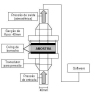
\includegraphics[width=9cm]{./figures/perm.pdf}
	\caption{Esquema de montagem do ensaio da medida de
    permeabilidade. \label{fig:perm}}
\end{figure}

   

\subsection{Resistência Mecânica}\label{mat:rm}
A resistência mecânica foi obtida através do ensaio de flexão em 3 pontos no
mesmo intervalo de temperaturas usado para a obtenção da porosidade e densidade
aparente, sendo realizados de acordo com a norma ASTM C133 utilizando 5 corpos
de prova no formato de paralelepípedos com dimensões de 25 x 25 x 150 mm$^3$. O
equipamento utilizado foi uma máquina de ensaios mecânicos universal (MTS,
Modelo 810, USA) usando uma taxa de carregamento constante de 12.9 N.s$^{-1}$. O
módulo de ruptura ($\sigma_f$) foi calculado pela Equação \ref{eq:modulo_rup}.

\begin{equation}
  \label{eq:modulo_rup}
  \sigma_f = \frac{3 \ P \ L}{2 \ b \ d^2}
\end{equation}

Onde $P$, é a carga de ruptura medida em N, L é a distância entre os apoios,
fixa em 127 mm; b é a largura e d , a altura do corpo de prova, sendo todas as
distâncias medidas em mm.
    
\subsection{Termogravimetria (TGA)}\label{mat:TGA}
    
Um dos principais ensaios para a simulação do processo de explosão durante o
processo de secagem em escala laboratorial é o ensaio de termogravimetria. O
sistema consiste em um forno com uma balança acoplada onde se mede a temperatura
da amostra e do forno além da evolução do peso de uma amostra cilíndrica com 40
mm de diâmetro e 40 mm de altura. Os corpos são aquecidos após cura a
30$^\circ$C por 24 horas. Foram utilizadas taxas de aquecimento constantes de
2$^\circ$C.min$^{-1}$, 5$^\circ$C.min$^{-1}$ e 20$^\circ$C.min$^{-1}$ no
intervalo de 30$^\circ$C e 800$^\circ$C. A perda de massa e sua taxa temporal
foram obtidas através das Equações \ref{eq:TGA_W} e \ref{eq:TGA_DTG}.

\begin{equation}
  \label{eq:TGA_W}
  W = \left( \frac{M_0-M}{M_0-M_f} \right) \ 100
\end{equation}

\begin{equation}
  \label{eq:TGA_DTG}
  DTG = \frac{\partial W}{\partial t}
\end{equation}

Onde $M_0$ é a massa inicial da amostra, $M$ é a massa observada num instante t,
e $M_f$ corresponde à massa final da amostra (todas medidas em gramas). $W$ é a
perda de massa percentual, enquanto DTG é a taxa de perda de massa (medida em
\%.min$^{-1}$). A Figura \ref{fig:TGA} apresenta o esquema de montagem do ensaio
de termogravimetria.
    
\begin{figure}[ht]
	\centering
	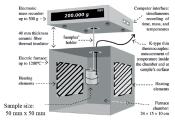
\includegraphics[width=9cm]{./figures/TGA.pdf}
	\caption{Esquema de montagem do ensaio de termogravimetria. \label{fig:TGA}}
\end{figure}



\subsection{Condutividade Térmica e Calor Específico}\label{mat:condutividade}
A condutividade térmica é obtida através do método do fio quente (com a
configuração dos fios paralelos) através do equipamento Netzsch TCT 426. A
medição se dá em um sistema de 3 tijolos com mesma composição dispostos um sobre
os outros. Entalhes de 0.4mm são realizados nos tijolos usando uma retífica
modelo Ferdimat T42 a fim de acomodar os fios do termopar.

A técnica obtém o valor de condutividade através de uma estimativa baseada no
tempo em que o calor gerado pelo fio quente (FQ) devido ao efeito Joule leva
para ser percebido no termopar da amostra ($T_a$) em uma condição de equilíbrio
térmico entra o conjunto de tijolos e o forno (através da medida de um termopar
de referência $T_r$). Tal ensaio permite a obtenção do calor específico através
da medida de difusividade térmica do material. A Figura \ref{fig:fio_quente}
apresenta o {\it layout} do ensaio.

\begin{figure}[!ht]
	\centering
	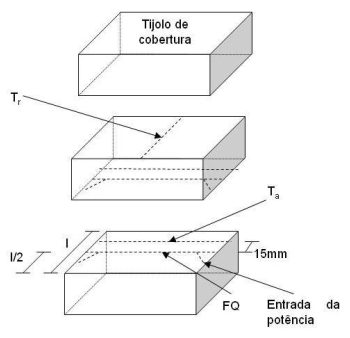
\includegraphics[width=9cm]{./figures/fio_quente.pdf}
	\caption{Esquema de montagem do ensaio da técnica de fio quente para obtenção
    da condutividade térmica e calor específico. \label{fig:fio_quente}}
\end{figure}

\section{Algoritmo de Otimização das Curvas de Secagem}\label{mat:pid}
A estratégia para obtenção de curvas de secagem otimizadas assemelha-se à
abordagem adotada por Fey et al \cite{Fey2017c}, na qual um controlador PID é
utilizado para controlar a temperatura a partir da pressão nos poros do
material. Assim, a abordagem em si não é baseada em um algoritmo de otimização,
no sentido no qual não se buscará um ótimo local ou global, mas sim buscará
ter-se o controle da pressão, evitando que seus níveis alcancem a resistência
mecânica do material, o que levaria a trincas ou explosões. O algoritmo funciona
a partir do cálculo de um erro $e$ entre a pressão máxima no interior dos poros
do material, $P_v^{max}$ , e a pressão máxima permitida $P_{max}$. Tal erro
dependerá do tempo e será recalculado em cada passo de tempo, conforme a Equação
\ref{eq:erro_pid}.

\begin{equation}
  \label{eq:erro_pid}
  e(t) = P_v^{max} - P_{max}
\end{equation}

Uma vez calculado o erro, é obtido a taxa de aquecimento instantânea (constante
naquele passo de tempo) ao qual a amostra será submetida, calculada segundo a
Equação \ref{eq:T_Rate}.

\begin{equation}
  \label{eq:T_Rate}
  \Delta T = K_{p} e(t)+K_{i} \int_{0}^{t} e(\tau) d \tau+K_{d} \frac{d e(t)}{d t}
\end{equation}

Uma das mais difíceis etapas para o uso de controladores PID é a definição das
constantes dos termos proporcional, integral e derivativo \cite{ogata2002}. No
presente trabalho, o refinamento de tais coeficientes foi realizado manualmente,
sendo $K_p = - 2.00 \ 10^{-6}$, $K_i= -6.25 \ 10^{-8}$ e $K_d = 0.00$, ou seja,
o termo derivativo utilizado é nulo, pois do contrário, as oscilações eram muito
elevadas.
 
  
%%% Local Variables:
%%% mode: latex
%%% TeX-command-extra-options: "-shell-escape"
%%% TeX-master: "TCC-Secagem"
%%% End:


% ----------------------------------------------------------
% Resultados e discussão
% ----------------------------------------------------------

\chapter{Resultados e discussão} \label{results}
\section{Propriedades}\label{sec:props}
As propriedades do material necessários para a simulação são a condutividade
térmica, o calor específico, a densidade, a permeabilidade e a água quimicamente
ligada contina na microestrutura do concreto, conforme apresentadas na Figura
\ref{fig:properties}.

 \begin{figure}[ht]
\centering
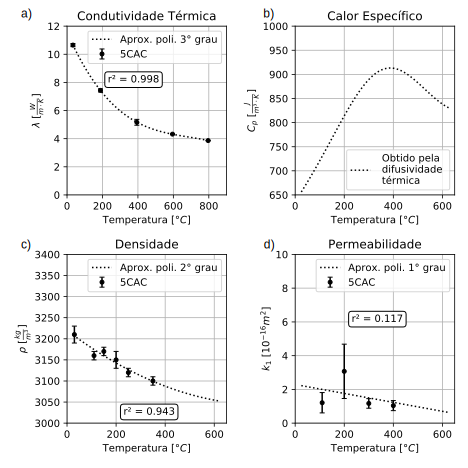
\includegraphics[width=14cm]{./figures/properties.pdf}
\caption{Caracterização da composição de concreto refratário utilizado no
  presente estudo, (a) condutividade térmica, (b) calor espicífico, (c)
  densidade e permeabilidade (d).  \label{fig:properties}}
\end{figure}

A condutividade térmica decai conforme a temperatura aumenta. Tal comportamento
pode ser aproximado por um polinômio de terceiro grau. Este comportamento
justifica-se pelo aumento da frequência de oscilações dos átomos, o que diminui
o caminho livre médio dos fónons, que são os principais transportadores de
energia térmica até aproximadamente 800$^\degree$C quando o transporte por
radiação começa a predominar \cite{pelissari2017}. A densidade é reduzida devido
a liberação da água físicamente adsorvida, bem como a água quimicamente ligada.
Outro efeito provável é a conversão de fases menos densas do cimento aluminoso
hidratado em fases de maior densidade, o que amplia a porosidade do material. O
calor específico foi calculado a partir da medida de difusividade térmica,
$\alpha = \frac{\lambda}{\rho \ C_p}$, e portanto não é apresentado o desvio
associado. Por fim, a permeabilidade do material apresenta um desvio padrão
muito elevado, e isto reflete no baixo valor de $r^2$ (aqui uma possível solução
seria aumentar o grau do polinômio, porém, seria o equivalente a realizar um {\it
  overfitting} uma vez que estaríamos inserindo no modelo um comportamento que
pode ser apenas o produto do erro da medida \cite{raschka2017}). 

 \begin{figure}[ht]
\centering
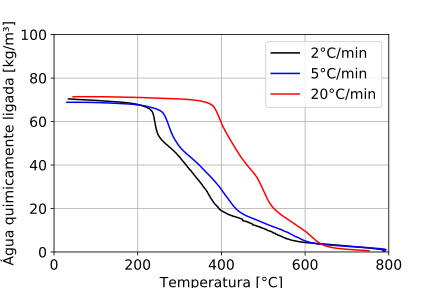
\includegraphics[width=14cm]{./figures/w_d.pdf}
\caption{Água quimicamente ligada por $m^3$ de concreto.  \label{fig:prop_wd}}
\end{figure}

Na Figura \ref{fig:prop_wd} a curva de liberação de água químicamente ligada é
apresentada. Sua medição é realizada a partir do ensaio de TGA realizado em
amostras previamente secas à 110$^\degree$C por 24 horas. Tal abordagem deve ser
considerada cuidadosamente, uma vez que sua precisão precisa ser investigada mais
a fundo. Uma possível problemática envolvida nessa maneira de medir a água de
desidratação é a formação de fases específicas durante a secagem a
110$^\degree$C, que não estariam presentes em uma secagem do material apenas
curado.



Uma útlima propriedade fundamental para o modelo são as curvas de sorção
isotérmicas que representam a quantidade de água evaporável (líquida e
adsorvida) no material. Tais medidas são complexas e segundo Baroghen-Bouny
\cite{baroghel2007water}, para se ter medidas confiáveis o método de medida deve
ser o método estacionário com soluções salinas para controle de umidade
relativa. Tais ensaios podem demorar meses até se atingir uma massa de água
adsorvida constante no material. Além da restrição de tempo, há uma notável
histerese quando comparado os comportamentos de sorção e adsorção que devem ser
levados em conta na medida. Como alternativa, há o uso do método dinâmico de
sorção de vapor, utilizado por Fey et al \cite{Fey2016b}, cuja validade das
medidas é limitado até 75\% de umidade relativa. Devido a indisponibilidade de
um equipamento capaz de realizar tais medidas, utilizou-se primeiramente a mesma
curva de sorção de Gong et al \cite{Gong1995a}, em seguida, devido ao desvio
apresentado, tal curva foi ajustada a fim de calibrar os resultados
experimentais com os resultados do modelo.

\section{Ensaios para o \textit{Benchmarking}}
A fim de realizar um benchmark do modelo, é proposto o uso do ensaio
termogravimétrico descrito na Seção \ref{metodologia}. A Figura
\ref{fig:TGA_measured} apresenta os resultados dos ensaios realizados à uma taxa
de 2$^\degree$C/min, 5$^\degree $C/min e 20$^\degree $C/min.

\begin{figure}[ht]
	\centering
	\includegraphics[width=12cm]{./figures/Mass_Loss.pdf}
	\caption{Resultado da perda de massa percentual dos ensaios de TGA realizados
    a taxas de 2$^\degree$ C/min, 5$^\degree$ C/min e 20$^\degree$ C/min.
  \label{fig:TGA_measured}}
\end{figure}

É possível observar que as taxas de perda de massa das amostras aquecidas à
2$^\degree$C/min e 5$^\degree$C/min são similares, com exceção ao intervalo de
100$^\degree$C à 270$^\degree$C (região onde se tem a maior parte de água
fisicamente adsorvida removida do sistema), especialmente após 300$^\degree$C,
assim como mostrado na Figura \ref{fig:prop_wd}. A amostra aquecida à
20$^\degree$C/min apresentou uma menor taxa de perda de massa para baixas
temperaturas, até a ocorrência da explosão por volta dos 290$^\degree$C.

\begin{figure}[ht]
	\centering
	\includegraphics[width=12cm]{./figures/DTG.pdf}
	\caption{Derivada da perda de massa percentual dos ensaios de TGA realizados
    a taxas de 2$^\degree$ C/min, 5$^\degree$ C/min e 20$^\degree$ C/min.
  \label{fig:DTG_measured}}
\end{figure}

A Figura \ref{fig:DTG_measured} apresenta os dados da derivada da curva de perda
de massa com respeito a temperatura. É possível observar que para a curva obtida
a partir do ensaio aquecido à 2$^\degree$C/min existem três picos distintos,
um em torno de 150$^\degree$C, outro em torno de 300$^\degree$C e o último em
torno de 475$^\degree$C. Tais picos podem estar associados com o regime de
evaporação e ebulição da água fisicamente adsorvida, e com as diferentes reações
de desidratação das fases de aluminato de cálcio hidratados
\cite{da2015refractory}.

O comportamento da amostra aquecida à 5$^\degree$C/min
é similar ao de 2$^\degree$C/min, com exceção ao fato de que o primeiro pico de
desidratação e o pico referente a saída da água fisicamente adsorvida não
apresentam uma clara separação. Tal comportamento poderia ser relacionado com um
atraso da remoção da água adsorvida, ocorrendo simultaneamente a liberação da
água fisicamente ligada e o início da desidratação (uma vez que a temperatura
para tal transformação sofre uma mudança muito pequena, conforme evidenciado na
Figura \ref{fig:prop_wd}).

Por fim, o ensaio realizado a 20$^\degree$C/min, explodiu antes de ocorrer o
início da desidratação das fases C$_3$AH$_6$ e da gibsita
\cite{da2015refractory} (i.e. Figura \ref{fig:prop_wd}), e portanto, é possível
concluir que sua explosão foi decorrente apenas da ebulição da água adsorvida.
Embora a presente conclusão concorde com os princípios de interpretação de
ensaios térmicos dinâmicos \cite{gabbott2008}, é importante salientar que a
correlação dos ensaios de TGA obtidos com amostras curadas (Figura
\ref{fig:TGA_measured}) com as amostras pré secadas à 110$^\degree$C (Figura
\ref{fig:prop_wd}), depende da hipótese de que durante tal pré-secagem não há
uma mudança de fases considerável a ponto de alterar a microestrutura do
material, mudando seu comportamento de desidratação.


\section{\textit{Benchmark} do modelo}
O modelo para a simulação da TGA foi feito através de uma malha tridimensional
com 33000 elementos, formando uma amostra cilíndrica de dimensões iguais ao do
corpo de prova utilizado no ensaio experimental (raio de 2,5 cm e altura de 5
cm). A fim de simular o aquecimento da amostra, toda a sua superfície lateral é
aquecida por radiação enquanto todas as faces são permeáveis, o incremento de
tempo utilizado foi de 30 segundos. A Figura \ref{fig:bench_setup} apresenta as
condições de contorno utilizadas.

As propriedades utilizadas foram obtidas na Seção \ref{sec:props} enquanto as
curvas de sorção foram ajustadas conforme descrito na Equação \ref{eq:mod_phi}. Tal ajuste
engloba não só a adequação da equação de estado (uma vez que em sua forma
original representava um concreto com cimento Portland \cite{bazant1979}) mas
também a soma de todos os erros experimentais de medida, bem como os efeitos das
simplificações e hipóteses adotadas no modelamento numérico apresentado no
Apêndice \ref{codigo}. Assim, a presente seção serve como um {\it benchmark}
qualitativo do modelo, sendo que seu uso para destintas geometrias necessitaria
de uma validação com outro ensaio, a fim de garantir que a resolução do problema
inverso resultasse em uma propriedade correta do material (i.e. invariante à
geometria e condições de contorno).

\begin{figure}[ht]
	\centering
	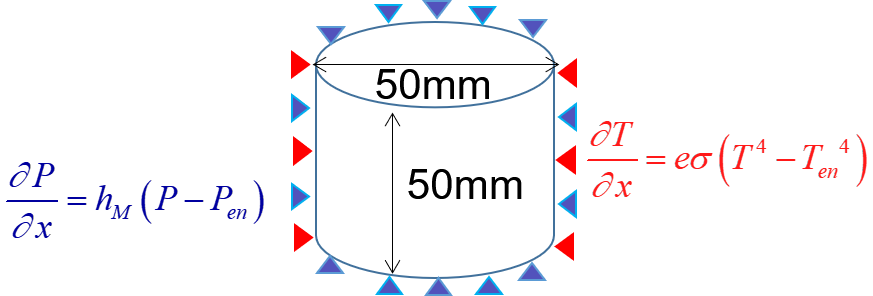
\includegraphics[width=12cm]{./figures/bench_setup.pdf}
	\caption{Geometria, dimensões e condições de contorno utilizadas no {\it benchmark}.
  \label{fig:bench_setup}}
\end{figure}

    \begin{equation}
      \label{eq:mod_phi}
      w(P, T) =
      \begin{cases} 
      w_c \left( \frac{w_0}{c} \ h(P,T) \right)^{\frac{1}{m(T)}} & h(P, T)\leq 0.6 \\
      w_{0.6} + (h(P, T) - 0.6) \frac{(w_{0.85} - w_{0.6})}{(0.85-0.6)} & 0.6 < h(P, T) < 0.85 \\
      w_c \ (0.04 \ (h(P, T) - 0.85) + 0.38 \ (1.1 - \frac{(T - 273.15)^2)}{1.8e5}) & 0.85 \leq h(P, T) 
      \end{cases}
    \end{equation}
 

A Figura \ref{fig:TGA_first} (a) apresenta a comparação entre as temperaturas
medidas pelo termopar próximo a superfície da amostra e as temperaturas da superfície do
modelo. É possível observar que há dois regimes distintos nas amostras aquecidas
à 2$^\degree$C/min e 5$^\degree$C/min. Um primeiro momento no qual
a taxa de aquecimento percebida pela amostra é maior nos dados experimentais do
que os dados do modelo (110 minutos para a amostra aquecida a 2$^\degree$C/min
70 minutos para a 5$^\degree$C/min) e um segundo momento, no qual o cenário se
inverte e a taxa de aquecimento percebida pela superfície da amostra
experimental é menor que a simulada.

\begin{figure}[!ht]
	\centering
	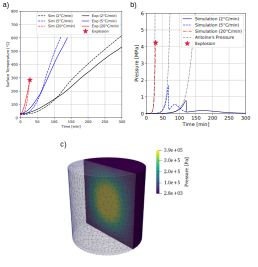
\includegraphics[width=14cm]{./figures/All_TGA_results.pdf}
	\caption{Evolução temporal da temperatura superficial, (a), da pressão máxima
    (b) e campo escalar de pressões ao final do ensaio da amostra simulada e
    aquecida à 5$^\degree$C/min, (c)).
  \label{fig:TGA_first}}
\end{figure}

Tal momento coincide com o fim da água fisicamente adsorvida, conforme é
possível observar na Figura \ref{fig:TGA_first} (b) que retrata a pressão máxima
em cada incremento de tempo da simulação. Conforme o arranjo experimental não
apresenta nenhum transdutor de pressão, tal resultado pode apenas ser comparado
com as curvas de pressão de saturação de Antoine, cujo os valores para a água
são tabelados \cite{yaws2006antoine}. Assim, é possível correlacionar que o fim
da água fisicamente adsorvida reduziu a quantidade de energia térmica necessária
para aumentar a temperatura da amostra fornecida ao sistema. Tal resultado será
referenciado para explicar os resultados seguintes. Por fim, é possível observar
que a amostra aquecida a 20$^\degree$C/min explodiu no momento em que a
simulação previa uma pressão de 4MPa, elevada o suficiente para causar uma
explosão, se estimarmos um módulo de Weibull de 7 e convertermos a resistência
mecânica à flexão três pontos do material (mensurada e valendo 6MPa) para a
resistência mecânica a tração pura (3MPa).

Por fim, a Figura \ref{fig:TGA_first} (c) apresenta todo o campo escalar de
pressões ao final do ensaio da amostra simulada e aquecida à 5$^\degree$C/min,
mostrando que o maior valor de pressão se encontra no centro da amostra.

Em seguida, a Figura \ref{fig:TGA_Mass} apresenta a comparação entre a massa
liberada do ensaio de TGA (curvas em vermelho) e a massa computada pela integral
da quantidade de água evaporável somada à água de desidratação (curva azul
escuro). A princípio é possível observar a mesma transição entre os regimes de
taxas de aquecimento observados nas Figuras \ref{fig:TGA_first} (a) e (b),
ocorrendo sempre a 200$^\degree$C, mostrando que a diferença de tempo entre as amostras
aquecidas a 2$^\degree$C/min e 5$^\degree$C/min é apenas decorrente do intervalo
de tempo necessário para se alcançar a temperatura de 200$^\degree$C.

Embora os resultados demonstrem certa concordância entre a simulação e os dados
experimentais, é possível observar que o ajuste manual da curva de sorção não
representou o comportamento demonstrado nas medidas experimentais, especialmente
da perda de massa em função da temperatura onde se pode ver que na simulação, a
água liberada em baixas temperaturas é muito maior do que a da medida
experimental (especialmente para o caso da amostra aquecida à 20$^\degree$C/min). 

\begin{figure}[H]
	\centering
	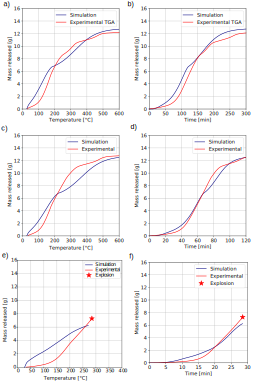
\includegraphics[width=14cm]{./figures/TGA_results_mass.pdf}
	\caption{Resultados de massa liberada em função da temperatura interna, (a),
    (b) e (c), e do tempo de simulação (d), (e) e (f).
  \label{fig:TGA_Mass}}
\end{figure}

\section{Otimização de uma curva de secagem}

A fim de demonstrar o potencial da ferramenta para a otimização da curva de
secagem, um caso fictício será apresentado. Trata-se da simulação da curva de
secagem de uma parede através do aquecimento unidirecional. As propriedades
utilizadas do material foram extraídas de Gong et al, \cite{Gong1995a} e o
modelo é baseado em uma malha unidimensional com 40 elementos lineares. As
condições de contorno são de aquecimento na face esquerda conforme a curva de
secagem, enquanto a face direita é resfriada por convecção natural em um
ambiente à 25$^\degree$C. A amostra é permeável em ambos os lados.

A Figura \ref{fig:No_PID} apresenta a curva de secagem (a), bem como a evolução
da pressão máxima na amostra (b). É possível observar que a pressão máxima
alcança um valor máximo de aproximadamente 10 bar (1.0 MPa, aqui a unidade
escolhida foi bar a fim de facilitar as comparações com o resultados reportados
por Gong) atingida durante o patamar. Tal resultado demonstra que o patamar está
mal dimensionado, uma vez que embora a pressão não cresça no intervalo de 2 a 4
horas, a água não é totalmente retirada, o que leva ao pico no tempo 6h.

\begin{figure}[H]
	\centering
	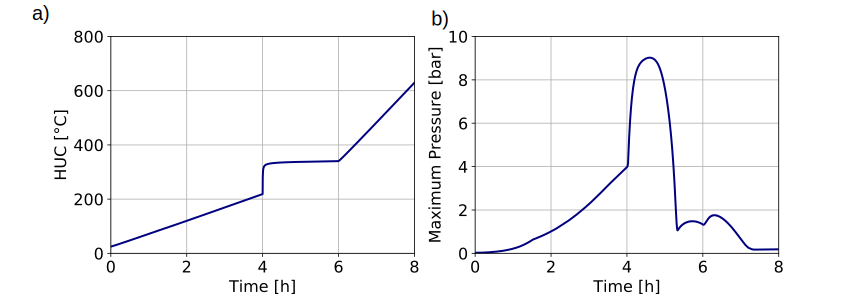
\includegraphics[width=14cm]{./figures/No_PID.pdf}
	\caption{Curva de aquecimento (a) e pressão máxima obtida (b) para o caso de referência.
  \label{fig:No_PID}}
\end{figure}

A fim de propor uma nova curva de secagem, no qual o patamar esteja dimensionado
corretamente, uma abordagem baseada no uso de um controlador do tipo PID,
conforme proposta por Fey et al, \cite{Fey2017c} e descrita na Seção
\ref{mat:pid}, foi utilizada. A pressão limite de 3 bar foi escolhida
arbitrariamente apenas a fim de mostrar o potencial da ferramenta. Como a taxa
de aquecimento do forno apresenta um limite máximo, no presente trabalho foi
necessário adicionar no algoritmo que o máxima taxa de aquecimento fosse de
150$^\degree$C/h (a mesma taxa máxima utilizada no caso anterior, de referência
sem o uso do controlador).


A Figura \ref{fig:PID} (a) apresenta a curva otimizada para a secagem. É
possível observar a existência de um patamar de duas horas na temperatura de
200$^\degree$C, sendo seguido por um forte aquecimento até a secagem completa do
material, conforme mostrado pela curva de pressão máxima (b). Também é possível
observar em (c) que o aquecimento da temperatura ambiente até 200$^\degree$C naõ foi
realizado a uma taxa constante, mas sim com uma taxa decrescente, de modo que a
pressão não excedesse tanto o limite de controle. Aqui é possível observar que o
algoritmo utilizado pelo controlador apresenta um {\it overshoot} de 1 bar
(conforme evidenciado em (d)). A presença de tal fenômeno se explica pelo
caráter dinâmico do problema, havendo uma certa inércia entre a atuação do
controlador e o seu efeito na resposta. Fey et al, no trabalho referenciado
resolveu tal problemática ao fazer uso de um segundo loop de controle,
adicionando um termo de erro proporcional à posição da pressão máxima, de forma
que fosse compensada e antecipada a ocorrência de {\it overshootings}.

\begin{figure}[H]
	\centering
	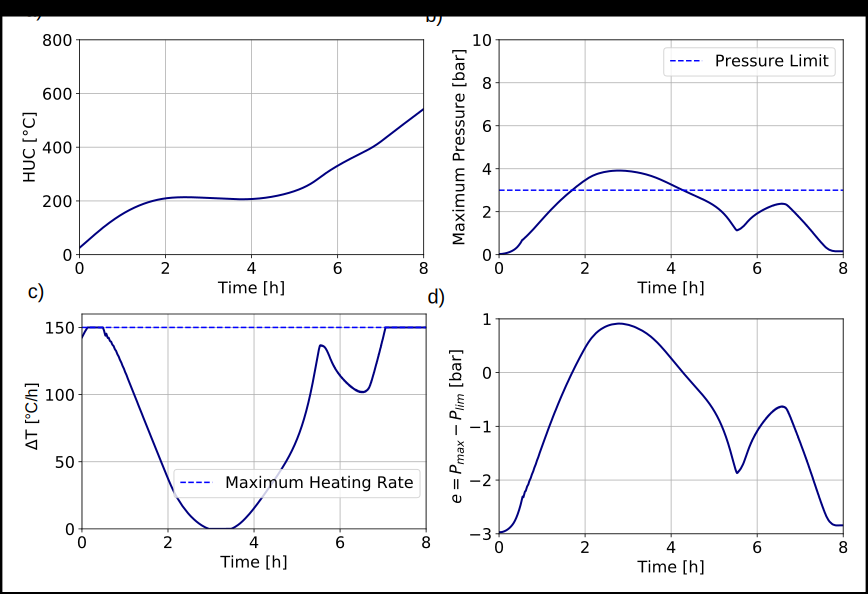
\includegraphics[width=14cm]{./figures/PID.pdf}
	\caption{Resultados de massa liberada em função da temperatura interna, (a),
    (b).
  \label{fig:PID}}
\end{figure}

No presente trabalho, tal estrutura complexa de algoritmo não foi contemplada
devido a limitações no tempo de desenvolvimento, e devido a possibilidade de se
contornar tal problemática utilizando um fator de segurança, uma vez que no
problema real a existência de um ``{\it undershoot}'' seria muito mais drástica
do que o uso de uma taxa de aquecimento mais conservadora, porém já otimizada
dada a geometria, o volume, as propriedades do material e as condições de
contorno do problema.

%%% Local Variables:
%%% mode: latex
%%% TeX-master: "TCC-Secagem"
%%% End:


% ---
% Finaliza a parte no bookmark do PDF, para que se inicie o bookmark na raiz
% ---
\bookmarksetup{startatroot}% 
% ---

% ---
% Conclusão
% ---
\chapter{Considerações finais} \label{conclusao}
\section{Conclusões do projeto}


\section{Trabalhos futuros}
O presente projeto pode ser encarado como uma experiência de sucesso, o objetivo
geral de se obter um modelo monofásico com baixo número de parâmetros capaz de
ser validade através do ensaio de TGA foi atingido, bem como os objetivos
específicos. Por outro lado, a baixa precisão quando comparado aos resultados
experimentais revelam a existência de novos desenvolvimentos que no contexto do
atual projeto não foram abordados. São eles:

\begin{itemize}
    \item Medidas experimentais das curva de sorção isotérmica;
    \item Propor um método de problema-inverso para obtenção da estimativa das
      curvas de sorção;
    \item Consideração de diversas camadas de materiais distintos;
    \item Implementação da formulação variacional para o problema mecânico;
    \item Realização de ensaios de TGA com amostras de diferentes tamanhos para
      considerar o efeito do volume da amostra;
    \item Reprodução dos ensaios de PTS (amostra aquecida unidimensionalmente com
      sensores de pressão, temperatura e medida da massa da amostra) e
      comparação com os dados de TGA;
    \item Estudo da presença de aditivos como fibras poliméricas e sua simulaçaõ
      em mesoescala;
    \item Acoplamento da um sistema controlador PID para a obtenção das curvas
      de sorção otimizadas para a redução da pressão gerada durante a secagem.
\end{itemize}

% ----------------------------------------------------------
% ELEMENTOS PÓS-TEXTUAIS
% ----------------------------------------------------------
\postextual


% ----------------------------------------------------------
% Referências bibliográficas
% ----------------------------------------------------------
\bibliography{bibliografia}

% ----------------------------------------------------------
% Glossário
% ----------------------------------------------------------
%
% Consulte o manual da classe abntex2 para orientações sobre o glossário.
%
%\glossary

% ----------------------------------------------------------
% Apêndices
% ----------------------------------------------------------

% ---
% Inicia os apêndices
% ---
\begin{apendicesenv}\label{apend}
\chapter{Código em Python} \label{codigo}

O presente trabalho baseia-se no modelo de Ba\v{z}ant \ref{sec:bazant}, assim
este apêndice tem como objetivo apresentar a implementação do problema
matemático através da plataforma FEniCS. Para tanto, é definida um caso a ser
simulado, escolhe-se a geometria e as condições de contorno para melhor
representar o problema físico. Em seguida é derivado o sistema de equações
parciais diferenciais em sua forma forte, este é então convertido em sua forma
fraca a qual é alimentada ao FEniCS e então realiza-se os calculos. Finalmente o
script é apresentado e a rotina de pós processamento definida.

    \section{Caso Ilustrativo}\label{mat:caso}
    O caso a ser simulado é uma seção transversal em 2 dimensões de uma parede
    de concreto refratário com espessura de 25 centímetros sujeita ao
    aquecimento por uma chama pelo seu lado esquerdo. A temperatura da chama é
    definida por uma curva de secagem que consiste em duas regiões de
    aquecimento separadas por um patamar de 5 horas. Do outro lado da parede há
    o meio ambiente com uma determinada temperatura fixa $T_{en}$. Assume-se que
    o transporte de massa se dá através de uma lei linear similar a Lei de
    Resfriamento de Newton. As faces superior e inferior da seção a ser simulada
    são consideradas adiabáticas resultando em planos de simetria. O setup pode
    ser visto na Figura \ref{fig:case}. A Tabela \ref{tab:case_ics_bcs}  resume
    as condições de contorno e as propriedades fictícias utilizadas.

  \begin{figure}[ht]
	\centering
	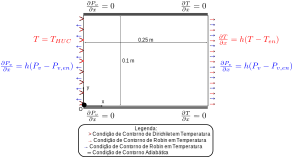
\includegraphics[width=14cm]{./figures/case.pdf}
	\caption{Esquema do caso ilustrativo apresentando as dimensões e condições de
    contorno aplicadas.  \label{fig:case}}
  \end{figure}

  \setlength{\tabcolsep}{38pt}
  
\begin{table}[]
\centering
\caption{Simulação do caso ilustrativo}
\label{tab:case_ics_bcs}
\addtolength{\tabcolsep}{-10pt}
\begin{tabular}{|ll|}
\hline
\multicolumn{2}{|l|}{Discretização no espaço e no tempo}                                    \\ \hline
Espessura da parede                                          & $L_x = 25 cm$                \\
Tempo simulado                                               & $t = 25 h$                   \\
Número de elementos em $x$                                   & $n_x = 50$                   \\
Número de elementos em $y$                                   & $n_y = 20$                   \\
Incremento de tempo                                          & $\Delta t = 15 s$            \\ \hline
\multicolumn{2}{|l|}{Condições Iniciais}                                                    \\ \hline
$T(x, y, t=0)$                                               & $ 25 ^{\circ}C$              \\
$P_v(x, y, t=0)$                                             & $ 2850 N \ m^{-2} $          \\ \hline
\multicolumn{2}{|l|}{Condições de Contorno}                                                 \\ \hline
$T(x=0, y, t)$                                               & $T_{HUC}(t)$                 \\
$\frac{\partial T}{\partial x}\bigg\rvert_{x = L_x, y, t}$   & $h \ (T - T_{en})$           \\
$\frac{\partial T}{\partial y}\bigg\rvert_{x, y=0, t}$       & $0$                          \\
$\frac{\partial T}{\partial y}\bigg\rvert_{x, y=L_y, t}$     & $0$                          \\
$\frac{\partial P_v}{\partial x}\bigg\rvert_{x = 0, y, t}$   & $h_m \ (P_v - P_{v, en})$    \\
$\frac{\partial P_v}{\partial x}\bigg\rvert_{x = L_x, y, t}$ & $h_m \ (P_v - P_{v, en})$    \\
$\frac{\partial P_v}{\partial y}\bigg\rvert_{x, y=0, t}$     & $0$                          \\
$\frac{\partial P_v}{\partial y}\bigg\rvert_{x, y=L_y, t}$   & $0$                          \\ \hline
\multicolumn{2}{|l|}{Propriedades}                                                          \\ \hline
Condutividade térmica do concreto refratário, $\lambda$      & $7 W \ m^{-1} \ K^{-1}$      \\
Densidade do concreto refratário, $\rho$                     & $2200 Kg \ m^{-3}$           \\
Calor específico do concreto refratário, $C_p$               & $1100 J \ Kg^{-1} \ K^{-1}$  \\
Curvas de Sorção Isotérmica, $w$                             & Equation \ref{eq:gong_phi}           \\
Permeabilidade, $K$                                          & Equation \ref{eq:baz_perm}           \\
Permeabilidade inicial, $K_0$                                & $ 10^{-12} m \ s^{-1}$       \\
Calor específico da água, $C_w$                              & $ 4100 J \ Kg^{-1} \ K^{-1}$ \\
Coeficiente de transferência de calor, $h$                   & $ 1 W \ m^{-2} \ K^{-1}$     \\
Coeficiente de transferência de calor, $h_m$                 & $ 1 \ 10^{-^6} s \ m^{-1}$   \\
Temperatura ambiente, $T_{en}$                               & $ 25 ^{\circ}C$              \\
Pressão Parcial de vapor de água, $P_{v, en}$                & $ 2850 N \ m^{-2} $          \\
Quantidade de cimento por Kg de concreto, $w_c$              & $ 300 Kg m^{-3} $            \\
Quantidade de água inicial por Kg de concreto, $w_0$         & $ 100 Kg m^{-3} $            \\ \hline
\end{tabular}
\end{table}

    A permeabilidade, ($K$), é retirada do modelo de Bažant, que também é utilizada pelo
    trabalho de Gong. Já a sorção isotérmica ($w$) é adaptada de \ref{eq:baz_phi}
    conforme descrito por Gong e representado pela Equação \ref{eq:gong_phi}.

\begin{equation}
  \label{eq:gong_phi}
      w(P, T) =
      \begin{cases} 
      w_c \left( \frac{w_0}{c} \ \phi(P,T) \right)^{\frac{1}{m(T)}} & \phi(P, T)\leq 0.96 \\
      w_{0.96} + (\phi(P, T) - 0.96) \frac{(w_{1.04} - w_{0.96})}{(1.04-0.96)} & 0.96 < \phi(P, T) < 1.04 \\
 w_c \ \left[0.037 (\phi-1.04) + 0.3335 \left(1 - \frac{T^2}{3.6 \ 10^5}) \right) \right] & \ 1.04 \leq \phi(P, T)
      \end{cases}
\end{equation}

    O uso de tal versão se justifica pois a equação é ajustada para a
    microestrutura de um concreto refratário \cite{Gong1995a} e ao não utilizar
    da porosidade, apresenta uma maior simplicidade de uso. Provido das
    propriedades apresentadas na Tabela \ref{tab:case_ics_bcs}, da geometria e
    das condições iniciais e de contorno, basta definir o sistema de equações a
    ser resolvido.

    \section{Sistema de Equações}\label{mat:eqs}
    Problemas de caráter transiente são modelos matemáticos cujas variáveis de
    resposta dependem do tempo. A solução de tais problemas através de modelos
    numéricos implica em uma discretização no tempo e no espaço. Há inúmeras
    estratégias para tal tarefa, porém no presente trabalho se utilizará de uma
    discretização espacial a partir de elementos finitos e temporal a partir de
    diferenças finitas.

    Conforme já apresentado na Seção \ref{sec:bazant}, a formulação se baseia no
    balanço de massa e energia dos fluxos de uma quantidade denominada umidade
    que representa tanto a água líquida livre, adsorvida e o vapor de água. A
    forma forte do sistema é composta pelas equações de balanço derivadas de
    \ref{eq:baz_MB} e \ref{eq:baz_EB}, pelas condições iniciais e de contorno. 
    
    \subsection{Forma Forte}\label{mat:forte}
    No presente modelo as variáveis independentes escolhidas são a temperatura
    $T$ e a pressão nos poros, $P_v$. A apresentação da formulação do problema em
    sua forma forte será descrito levando em consideração funções não explicítas
    das variaveis independentes a fim de simplificar as expressões matemáticas.

    
    Substituindo as Equações \ref{eq:Darcy}, \ref{eq:Fourier} nas
    Equações  \ref{eq:baz_MB} e \ref{eq:baz_EB} obtém-se o problema em sua forma
    forte:  

    Equações de Conservação:
   \begin{equation}
     \label{eq:full_MB}
     \frac{\partial w}{\partial t}  = \nabla \cdot \left(\frac{K}{g} \nabla P_v \right) + \frac{\partial w_d}{\partial t} \ \text{in } \Omega
   \end{equation}

   \begin{equation}
      \label{eq:full_EB}
      \frac{\partial T}{\partial t} = C_a \ \frac{\partial w}{\partial t} +  C_w \frac{K}{g} \ \nabla P_v \cdot \nabla T + \nabla \cdot (\lambda \nabla T) \ \text{in } \Omega
   \end{equation}

   Condição de contorno de Dirichlet:
   \begin{equation}
     \label{eq:dir_bc}
    T(0, y, t) = T_{HUC}(t) \ \text{in } \Gamma_D
   \end{equation}

   Condições de contorno de Neumann:
   \begin{equation}
     \label{eq:neu_bc_T_x}
     \frac{\partial T}{\partial x}\bigg\rvert_{x = L_x, y, t} =  (T - T_{en}) \ \text{in } \Gamma_{N, T_{env}}
   \end{equation}

   \begin{equation}
     \label{eq:neu_bc_T_y}
\frac{\partial T}{\partial y}\bigg\rvert_{x, y=0, t} = \frac{\partial T}{\partial y}\bigg\rvert_{x, y=L_y, t} = 0 \ \text{in } \Gamma_{N, adi}
   \end{equation}

   
   \begin{equation}
     \label{eq:neu_bc_P_x}
     \frac{\partial P_v}{\partial x}\bigg\rvert_{x = 0, y, t} = \frac{\partial P_v}{\partial x}\bigg\rvert_{x = L_x, y, t} =  h_m \ (P_v - P_{v, en}) \ \text{in } \Gamma_{N, P_{env}}
   \end{equation}

   \begin{equation}
     \label{eq:neu_bc_P_y}
    \frac{\partial P_v}{\partial y}\bigg\rvert_{x, y=0, t}= \frac{\partial P_v}{\partial y}\bigg\rvert_{x, y=L_y, t} = 0 \ \text{in }\Gamma_{N, adi}
   \end{equation}


   
    Deve-se salientar que as derivadas temporais das curvas de sorção são
    obtidas a seguir como função das derivadas parciais das variáveis
    independentes. Tal abordagem permite expressar o problema em termos mais simples.

    \begin{equation}
      \label{eq:dwdt}
      \frac{\partial w}{\partial t} = \frac{\partial w}{\partial P_v} \frac{\partial P_v}{\partial t} + \frac{\partial w}{\partial T} \frac{\partial T}{\partial t}
    \end{equation}

    Além disso, as derivadas temporais das variáveis independentes são aproximadas
    por diferenças finitas anteriores conforme descrito pelas Equações \ref{eq:fd_P} e \ref{eq:fd_T}.

    \begin{equation}
      \label{eq:fd_P}
      \frac{\partial P_v}{\partial t} = \frac{P_v - P_v^n}{\Delta t}
    \end{equation}
    
    \begin{equation}
      \label{eq:fd_T}
      \frac{\partial T}{\partial t} = \frac{T - T^n}{\Delta t}
    \end{equation}

    Por fim, as derivadas parciais das curvas de sorção isotérmica são
    aproximadas por diferenças finitas centrais, Equações \ref{eq:fc_P} e \ref{eq:fc_T}.

    \begin{equation}
      \label{eq:fc_P}
      \frac{\partial w}{\partial P_v^n} = \frac{w(P_v^n+\delta \ P_v^n, \ T^n)- w(P_v^n- \delta \ P_v^n , \ T^n)}{2 \ \delta}
    \end{equation}

    
    \begin{equation}
      \label{eq:fc_T}
      \frac{\partial w}{\partial T^n} = \frac{w(P_v^n, \ T^n+\delta \ T^n)- w(P_v^n, \ T^n- \delta \ T^n)}{2 \ \delta}
    \end{equation}

    Onde $\delta$ é um diferencial numérico com valor $\delta = 0.0001$.

    
    \subsection{Forma Fraca}\label{mat:fraca}
    A forma fraca é obtida a partir da multiplicação das equações de conservação
    de massa e de energia pela função teste $\psi$ e subsequente integração
    sobre o domínio numérico. É utilizada a identidade de Green quando aplicável
    para se obter a forma fraca final.

  \begin{equation}
     \label{eq:weak_MB}
  \int_{\Omega}  \frac{\partial w}{\partial t} \ \psi \ \text{d}x =   \int_{\Omega}    \frac{K}{g} \left(  \nabla P_v \cdot \nabla  \psi \right) \ \text{d}x +   \int_{\Omega}    \frac{\partial w_d}{\partial t}  \ \psi \ \text{d}S \ +   \int_{\Gamma_{N, P_{env}}} \left( P_v \cdot \mathbf{n} \right) \ \psi \ \text{in } \Omega
   \end{equation}

   \begin{eqnarray}
     \label{eq:weak_EB}
      \int_{\Omega} \frac{\partial T}{\partial t} \ \psi \ \text{d}x &=&
                                                                         \int_{\Omega}
                                                                         C_a \
                                                                         \frac{\partial
                                                                         w}{\partial
                                                                         t} \
                                                                         \psi \
                                                                         \text{d}x
                                                                         +
                                                                         \int_{\Omega}
                                                                         C_w
                                                                         \frac{K}{g}
                                                                         \
                                                                         \nabla
                                                                         P_v
                                                                         \cdot
                                                                         \nabla
                                                                         T \
                                                                         \psi \
                                                                         \text{d}x
     \nonumber \\
                                                                         & &+ \int_{\Omega} \lambda \ \nabla T \cdot \nabla \psi \ \text{d}x + \int_{\Gamma_{T_{env}}} \left( T \cdot \mathbf{n} \right) \ \psi \ \text{d}x \ \text{in } \Omega
    \end{eqnarray}

    
    Tal sistema é fornecido à biblioteca FEniCS que converte o sistema de
    equações parciais diferenciais em um sistema linear de equações baseado nas
    funções de forma escolhidas. Esse sistema é resolvido iterativamente e o
    resultado é obtido através dos valores nodais (em cada um dos nós da malha
    que representa a discretização da geometria do problema) das variáveis de interesse.

    A seguir será delineado a estrutura do código apresentando uma clara
     correlação com cada etapa da descrição matemática.
     
    \section{Estrutura do script}\label{mat:script}
    O script pode ser separado nas seguintes etapas:

    \begin{itemize}
    \item Importação das bibliotecas necessárias
    \item Definição dos parâmetros de discretização temporal e espacial
    \item Definição da malha a partir da geometria
    \item Especificação das condições de contorno
    \item Definição dos espaços das funções de elementos finitos
    \item Definição das propriedades dos materiais
    \item Especificação das condições iniciais
    \item Descrição do sistema de equações em sua forma fraca
    \item Loop temporal de resolução das equações e armazenamento dos resultados 
    \end{itemize}

    Cada uma das etapas serão detalhadas e o código mostrado.

    
    \subsection{Importação das bibliotecas}
    Para a simulação, apenas o pacote \mintinline[bgcolor=bg]{python}{dolfin} da biblioteca
    FEniCS é necessário. O pacote \mintinline[bgcolor=bg]{python}{datetime} é utilizado para
    contabilizar o tempo decorrido de simulação. Já os pacotes
    \mintinline[bgcolor=bg]{python}{csv} e \mintinline[bgcolor=bg]{python}{os} são importados para
    salvar as séries temporais de variáveis de interesse em uma planilha e para 
    gerenciar em qual diretório serão salvos os arquivos, respectivamente.

    \begin{minted}[
      frame=lines,
      framesep=2mm,
      baselinestretch=1.2,
      bgcolor=bg,
      fontsize=\footnotesize,
      linenos
      ]{python}

      from dolfin import *
      from datetime import datetime
      import csv
      import os
    \end{minted}
   
    \subsection{Definição da discretização}
    Conforme definido na Tabela \ref{tab:case_ics_bcs}, a discretização é
    definida a partir das seguintes variáveis.
    
    \begin{minted}[
      frame=lines,
      framesep=2mm,
      baselinestretch=1.2,
      bgcolor=bg,
      fontsize=\footnotesize,
      linenos
      ]{python}
      
      # Time discretization
      t = 0
      T_total = 25 * 3600
      dt = 15
      
      # Space discretization
      lx = 0.25
      ly = 0.10
      Nx = 50
      Ny = 20
    \end{minted} 

    \subsection{Definição da malha e das condições de contorno}
    O pacote FEniCS já vem com uma ferramenta capaz de gerar malhas em
    geometrias simplistas. Dessa forma, para definir a malha da seção retangular
    da parede do caso de estudo é simples utilizando apenas a função
    \mintinline[bgcolor=bg]{python}{RectangleMesh()}. Em seguida, cria-se um
    objeto que representa as condições de contorno através da função
    \mintinline[bgcolor=bg]{python}{MeshFunction()}, cujos argumentos definem
    qual o tipo desse contorno (face interna ou externa), a malha, e a dimensão
    do contorno (pontos para um domínio unidimensional, curvas para domínios
    bidimensionais e superfícies para domínios tridimensionais). Por fim, é
    criada uma classe para cada parede do retângulo. Tais classes são utilizadas
    para marcar uma bandeira em cada nó que pertence a tais contornos. Por fim é
    criada uma medida através da função \mintinline[bgcolor=bg]{python}{Measure()} que será utilizada na formulação da forma fraca.
    
    \begin{minted}[
      frame=lines,
      framesep=2mm,
      baselinestretch=1.2,
      bgcolor=bg,
      fontsize=\footnotesize,
      linenos
      ]{python}

      # Mesh and Boundaries Condition Definitions
      mesh = RectangleMesh(0.0, 0.0, lx, ly, Nx, Ny)

      # Boundaries
      boundaries = MeshFunction('size_t', mesh, mesh.topology().dim() - 1)
      boundaries.set_all(0)


      class left(SubDomain):
          def inside(self, x, on_boundary):
              return abs(x[0]) < DOLFIN_EPS and on_boundary
      

      class right(SubDomain):
          def inside(self, x, on_boundary):
              return abs(x[0] - lx) < DOLFIN_EPS and on_boundary


      class top(SubDomain):
          def inside(self, x, on_boundary):
              return abs(x[1] - ly) < DOLFIN_EPS and on_boundary


      class down(SubDomain):
          def inside(self, x, on_boundary):
              return abs(x[1]) < DOLFIN_EPS and on_boundary


      left = left()
      right = right()
      top = top()
      down = down()
      left.mark(boundaries, 1)
      right.mark(boundaries, 2)
      top.mark(boundaries, 3)
      down.mark(boundaries, 4)
      ds = Measure("ds", domain=mesh, subdomain_data=boundaries)
    \end{minted} 

    \subsection{Definição dos espaços das funções de elementos finitos}
    Uma vez definida as geometrias do problema, criam-se o espaço da função de
    elementos finitos onde residem as funções teste e as funções bases que
    aproximação as variáveis independentes do problema (a temperatura e a
    pressão). Como o problema é acoplado de maneira forte, o espaço vetorial
    deverá compreender elementos que aproximem ambas as funções e para tanto
    cria-se um espaço misto. Para tanto, é criado primeiramente um objeto que
    representa um elemento finito linear
    \mintinline[bgcolor=bg]{python}{RectangleMesh(P1)}. Em seguida define-se o
    elemento misto e o espaço de função sobre a malha usando a
    função\mintinline[bgcolor=bg]{python}{FunctionSpace()}. A partir daí é
    possível obter funções teste e funções de aproximação a partir do espaço V.  
    
     \begin{minted}[
      frame=lines,
      framesep=2mm,
      baselinestretch=1.2,
      bgcolor=bg,
      fontsize=\footnotesize,
      linenos
      ]{python}
     # Mixed element and space functions definition
     P1 = FiniteElement('P', mesh.ufl_cell(), 1)
     element = MixedElement([P1, P1])
     V = FunctionSpace(mesh, element)
     v_1, v_2 = TestFunctions(V)
     u = Function(V)
     P_v, T = split(u)
     u_n = Function(V)
     P_v_n, T_n = split(u_n)

    \end{minted} 
   
    \subsection{Definição das propriedades do material}
    Cada uma das propriedades são definidas através de funções definidas em
    python. A única especificidade referente ao uso da plataforma FEniCS é o uso
    de uma função própria para definir condicionais. 

    \subsection{Especificação das condições iniciais}
    As condições iniciais são projetadas no espaço de elementos finitos usando a
    função \mintinline[bgcolor=bg]{python}{interpolate()}.
    
    \begin{minted}[
      frame=lines,
      framesep=2mm,
      baselinestretch=1.2,
      bgcolor=bg,
      fontsize=\footnotesize,
      linenos
      ]{python}
     
     # Initial conditions
     P_0 = P_v_inf
     P_v_n = interpolate(P_0, V.sub(0).collapse())
     T_0 = Constant(298.15)
     T_n = interpolate(T_0, V.sub(1).collapse())
    \end{minted} 

    \subsection{Descrição da forma fraca}
    Em seguida, a forma fraca é definida. Na presente subseção também será
    criado um objeto que representa o problema numérico a ser resolvido.
    A representação é direta do problema descrito em \ref{mat:fraca}. A
    integração é apenas representada implicitamente pela
    multiplicação de cada termo pela medida volumétrica
    \mintinline[bgcolor=bg]{python}{dx} ou de contorno
    \mintinline[bgcolor=bg]{python}{ds}.

    Também se define o Jacobiano do resíduo que será utilizado no algoritmo de
    resolução através do método de Newton. Por fim, são definidos objetos que
    representam o problema numérico (\mintinline[bgcolor=bg]{python}{problem}) e o algoritmo de solução em si (\mintinline[bgcolor=bg]{python}{solver}).
    
    \begin{minted}[
      frame=lines,
      framesep=2mm,
      baselinestretch=1.2,
      bgcolor=bg,
      fontsize=\footnotesize,
      linenos
      ]{python}

     # Variational formulation in residual form
     # Mass balance equation equation
     ResP = dwdt(P_v, T, P_v_n, T_n) * v_1 * dx
     ResP += (a(P_v_n, T_n) / g) * inner(nabla_grad(P_v), nabla_grad(v_1)) * dx
     ResP += - ((w_d(T) - w_d(T_n)) / dt) * v_1 * dx
     ResP += B_w * (P_v - P_v_inf) * v_1 * (ds(1) + ds(2) + ds(3) + ds(4))


     # Energy balance equation
     ResT = rho * C_p * ((T - T_n) / dt) * v_2 * dx
     ResT += k * inner(nabla_grad(T), nabla_grad(v_2)) * dx
     ResT += - h_d * ((w_d(T) - w_d(T_n)) / dt) * v_2 * dx
     ResT += - C_a(T_n) * dwdt(P_v, T, P_v_n, T_n) * v_2 * dx
     ResT += C_w * (a(P_v_n, T_n) / g) * \
         inner(nabla_grad(P_v_n), nabla_grad(T_n)) * v_2 * dx
     ResT = ResT + (B_t * (T - T_inf) +
                   C_a(T_n) * B_w * (P_v - P_v_inf)) * v_2 * (ds(2) + ds(3))


     # Total residual
     Res = ResT + ResP

     # Jacobian
     Jac = derivative(Res, u)
     problem = NonlinearVariationalProblem(Res, u, bcs, Jac, ffc_options)
     solver = NonlinearVariationalSolver(problem)
    \end{minted} 

    \subsection{Loop temporal}
    Em seguida, após a definição do problema e do objeto que representa o
    algoritmo de solução cria-se um loop que deverá rodar até o tempo de
    simulação alcançar o tempo total simulado (25 h). A evolução da pressão
    máxima, da temperatura máxima e da quantidade de água livre do sistema são
    salvos em um arquivo .csv que permite sua visualização online (i.e. durante
    a simulação).

    Ao entrar no loop o tempo atual de simulação é utilizado para
    definir em qual etapa da curva de aquecimento se está. Isto define a
    temperatura na condição de contorno de Dirichlet. Em seguida é resolvido o
    sistema linear de equações. A quantidade de água livre no sistema é
    integrada ao longo do domínio e os valores do timestep anterior são
    igualados ao timestep atual. A cada dez ciclos dentro do loop os resultados
    de todo o domínio são salvos em um arquivo que pode ser visualizado através
    da plataforma Paraview \cite{paraview2007}. O tempo de simulação é corrigido e o ciclo se
    inicia novamente.

    Ao alcançar o tempo total de simulação o programa saí do loop, o arquivo csv
    é salvo e se calcula o tempo real gasto pela simulação.
    
     \begin{minted}[
      frame=lines,
      framesep=2mm,
      baselinestretch=1.2,
      bgcolor=bg,
      fontsize=\footnotesize,
      linenos
      ]{python}
     f = open(dir_ + '/time_series.csv', 'w')
     writer = csv.writer(f, delimiter='\t')
     startTime = datetime.now()
     while t <= T_total:

         print('Progress: ' + str(round(t / T_total * 100, 2)) + '%')
     
         # Solve non-linear problem
         T_huc.t = t
         if t < 5 * 3600:
             T_huc.rate = 50
             T_huc.T_0 = 298.15
         elif (t > 5 * 3600) & (t < 10 * 3600):
             T_huc.rate = 0
             T_huc.T_0 = 298.15 + 250
         elif (t > 10 * 3600):
             T_huc.rate = 30
             T_huc.t_0 = 15.833 * 3600
             T_huc.T_0 = 298.15 + 250

         n, conv = solver.solve()

         # integration over domain of water quantity
         wat = assemble((w(P_v_n, T_n)) * dx,
                        form_compiler_parameters=ffc_options)
         w_domain.append(wat)
         convergence.append(n)
         time.append(t)

         # Update solution with last computed value
         (_P, _T) = u.split(True)
         P_v_n.vector()[:] = _P.vector()
         T_n.vector()[:] = _T.vector()
         P_v_max = max(P_v_n.vector()[:]) / 1e6
         P_v_min = min(P_v_n.vector()[:]) / 1e6
         T_max = max(T_n.vector()[:])
         T_min = min(T_n.vector()[:])

         writer.writerow([t, H, wat, n, T_max, P_v_max])

         if (nt % freq_out == 0):
             _P.rename("Pressure [Pa]", "P_v")
             _T.rename("Temperature [K]", "T")
             filex.write(_P, t)
             filex.write(_T, t)

         nt += 1
         t += dt
     # End loop over time steps
     f.close()
     time_delta = datetime.now() - startTime
     print('Simulation time: ', str(time_delta))
    \end{minted} 
   
    \section{Pós-processamento}
    O pós processamento se dá através de dois tipos de dados principais, são
    eles o arquivo csv que tem como objetivo dar um indicativo qualitativo da
    convergência correta da simulação (isto é, se o resultado é condizente, se a
    temperatura de aquecimento é obedecida, se a pressão máxima é um valor
    coerente ou se a quantidade de água está seguindo o comportamento já
    esperdo), e os dados nodais de todo o domínio.

    Os dados do domínio são os mais importantes porém resultam em arquivos
    pesados (dependendo do refinamento da malha e do tamanho do incremento de
    tempo). Portanto dependendo da simulação o intervalo de registro dos dados
    pode ser maior ou menor. Análises qualitativas são realizadas usando o
    Paraview enquanto análises quantitativas, descritas em termos de gráficos da
    evolução de propriedade em diferentes posições ou de perfis térmicos em
    diferentes tempos, são obtidos por rotinas em Python.




\end{apendicesenv}
% ---


% ----------------------------------------------------------
% Anexos
% ----------------------------------------------------------

% ---
% Inicia os anexos
% ---
%\begin{anexosenv}
%\chapter{Anexo} \label{orcamento}

%\includepdf[pages=1-2]{DFA100.pdf}
%\end{anexosenv}

%---------------------------------------------------------------------
% INDICE REMISSIVO
%---------------------------------------------------------------------

\printindex

\end{document}

% Local Variables:
% TeX-command-extra-options: "-shell-escape"
% End:
